\documentclass[12pt]{article}%
%%%%%%%%%%%%%%%%%%%%%%%%%%%%%%%%%%%%%%%%%%%%%%%%%%%%%%%%%%%%%%%%%   
% All style files are available from 
%   http://wwww.uiuc.edu/~sariel/research/latex/
%%%%%%%%%%%%%%%%%%%%%%%%%%%%%%%%%%%%%%%%%%%%%%%%%%%%%%%%%%%%%%%%%%   


%%%%%%%%%%%%%%%%%%%%%%%%%%%%%%%%%%%%%%%%%%%%%%%%%%%%%%%%%%%%%%%%%%   
% Conditional compilation depending on whether this is my computer or
% not.
\IfFileExists{sariel_computer.sty}{\def\sarielComp{1}}{}
\ifx\sarielComp\undefined%
\newcommand{\SarielComp}[1]{}
\newcommand{\NotSarielComp}[1]{#1}%
\else
\newcommand{\SarielComp}[1]{#1}%
\newcommand{\NotSarielComp}[1]{}%
\fi
\newcommand{\IfPrinterVer}[2]{#2}%

%%%%%%%%%%%%%%%%%%%%%%%%%%%%%%%%%%%%%%%%%%%%%%%%%%%%%%%%%%%%%%%%%% 


\usepackage[cm]{fullpage}%
\usepackage{amsmath}%
\usepackage{amssymb}%
\usepackage[cmyk]{xcolor}%
%\usepackage{xcolor}%

\SarielComp{\usepackage{sariel_colors}}%

\usepackage[amsmath,thmmarks]{ntheorem}%
\theoremseparator{.}%

\usepackage{titlesec}%
\titlelabel{\thetitle. }%

\usepackage{graphicx}%
\usepackage{xcolor}%
\usepackage{mleftright}%
\usepackage{xspace}%
\usepackage{hyperref}%

\usepackage{caption}%

\newcommand{\hrefb}[3][black]{\href{#2}{\color{#1}{#3}}}%

\IfPrinterVer{%
   \usepackage{hyperref}%
}{%
   \usepackage{hyperref}%
   \hypersetup{%
      breaklinks,%
      ocgcolorlinks, colorlinks=true,%
      urlcolor=[rgb]{0.25,0.0,0.0},%
      linkcolor=[rgb]{0.5,0.0,0.0},%
      citecolor=[rgb]{0,0.2,0.445},%
      filecolor=[rgb]{0,0,0.4},
      anchorcolor=[rgb]={0.0,0.1,0.2}%
   }
   % \usepackage{cleveref}
}

% ----------------------------------------------------------------------
% ----------------------------------------------------------------------
% Defining theorem like environments
% ----------------------------------------------------------------------
% ----------------------------------------------------------------------
\theoremseparator{.}%

\theoremstyle{plain}%
\newtheorem{theorem}{Theorem}[section]

\newtheorem{lemma}[theorem]{Lemma}
\newtheorem{conjecture}[theorem]{Conjecture}
\newtheorem{corollary}[theorem]{Corollary}
\newtheorem{claim}[theorem]{Claim}%
\newtheorem{fact}[theorem]{Fact}
\newtheorem{observation}[theorem]{Observation}
\newtheorem{invariant}[theorem]{Invariant}
\newtheorem{question}[theorem]{Question}
\newtheorem{proposition}[theorem]{Proposition}
\newtheorem{prop}[theorem]{Proposition}
\newtheorem{openproblem}[theorem]{Open Problem}

\theoremstyle{plain}%
\theoremheaderfont{\sf} \theorembodyfont{\upshape}%
\newtheorem*{remark:unnumbered}[theorem]{Remark}%
\newtheorem*{remarks}[theorem]{Remarks}%
\newtheorem{remark}[theorem]{Remark}%
\newtheorem{definition}[theorem]{Definition}
\newtheorem{defn}[theorem]{Definition}
\newtheorem{example}[theorem]{Example}
\newtheorem{exercise}[theorem]{Exercise}
\newtheorem{problem}[theorem]{Problem}
\newtheorem{xca}[theorem]{Exercise}
\newtheorem{exercise_h}[theorem]{Exercise}
\newtheorem{assumption}[theorem]{Assumption}%

% Proof environment
\newcommand{\myqedsymbol}{\rule{2mm}{2mm}}

\theoremheaderfont{\em}%
\theorembodyfont{\upshape}%
\theoremstyle{nonumberplain}%
\theoremseparator{}%
\theoremsymbol{\myqedsymbol}%
\newtheorem{proof}{Proof:}%

\newtheorem{proofof}{Proof of\!}%

% theorem block end
%%%%%%%%%%%%%%%%%%%%%%%%%%%%%%%%%%%%%%%%%%%%%%%%%%%%%%%%%%%%%%%%%%%%


%%%%%%%%%%%%%%%%%%%%%%%%%%%%%%%%%%%%%%%%%%%%%%%%%%%%%%%%%%%%%%%%%% 5
% Color emph
\providecommand{\emphind}[1]{\emph{#1}\index{#1}}
\definecolor{nalmostblack}{rgb}{0, 0, 0.7}
\providecommand{\emphic}[2]{%
   \textcolor{nalmostblack}{%
      \textbf{\emph{#1}}}%
   \index{#2}}


\providecommand{\emphi}[1]{\emphic{#1}{#1}}

\definecolor{almostblack}{rgb}{0, 0, 0.5}
\providecommand{\emphw}[1]{{\emph{{\textcolor{almostblack}{#1}}}}}%

\providecommand{\emphOnly}[1]{\emph{\textcolor{almostblack}{\textbf{#1}}}}
% Color emph - end 
%%%%%%%%%%%%%%%%%%%%%%%%%%%%%%%%%%%%%%%%%%%%%%%%%%%%%%%%%%%%%%%%%% 5


\numberwithin{figure}{section}%
\numberwithin{table}{section}%
\numberwithin{equation}{section}%


%%%%%%%%%%%%%%%%%%%%%%%%%%%%%%%%%%%%%%%%%%%%%%%%%%%%%%%%%%%%%%%%%%%
% Sariel's thanks
%%%%%%%%%%%%%%%%%%%%%%%%%%%%%%%%%%%%%%%%%%%%%%%%%%%%%%%%%%%%%%%%%%% 

\providecommand{\tildegen}{{\protect\raisebox{-0.1cm}
      {\symbol{'176}\hspace{-0.01cm}}}}
\newcommand{\atgen}{\symbol{'100}}
\newcommand{\SarielThanks}[1]{\thanks{Department of Computer Science;
      University of Illinois; 201 N. Goodwin Avenue; Urbana, IL,
      61801, USA; {\tt sariel\atgen{}illinois.edu}; {\tt
         \url{http://sarielhp.org/}.} #1}}


%%%%%%%%%%%%%%%%%%%%%%%%%%%%%%%%%%%%%%%%%%%%%%%%%%%%%%%%%%%%%%%%%%%%%%
%    Handling references
%%%%%%%%%%%%%%%%%%%%%%%%%%%%%%%%%%%%%%%%%%%%%%%%%%%%%%%%%%%%%%%%%%%%%%

\newcommand{\HLink}[2]{\hyperref[#2]{#1~\ref*{#2}}}
\newcommand{\HLinkSuffix}[3]{\hyperref[#2]{#1\ref*{#2}{#3}}}

\newcommand{\figlab}[1]{\label{fig:#1}}
\newcommand{\figref}[1]{\HLink{Figure}{fig:#1}}

\newcommand{\thmlab}[1]{{\label{theo:#1}}}
\newcommand{\thmref}[1]{\HLink{Theorem}{theo:#1}}

\newcommand{\corlab}[1]{\label{cor:#1}}
\newcommand{\corref}[1]{\HLink{Corollary}{cor:#1}}%

\providecommand{\deflab}[1]{\label{def:#1}}
\newcommand{\defref}[1]{\HLink{Definition}{def:#1}}


\newcommand{\clmlab}[1]{\label{claim:#1}}
\newcommand{\clmref}[1]{\HLink{Claim}{claim:#1}}

\newcommand{\apndlab}[1]{\label{apnd:#1}}
\newcommand{\apndref}[1]{\HLink{Appendix}{apnd:#1}}

\newcommand{\seclab}[1]{\label{sec:#1}}
\newcommand{\secref}[1]{\HLink{Section}{sec:#1}}
\newcommand{\rectA}{\Mh{B}}%
\newcommand{\rectB}{\Mh{D}}%
\newcommand{\clientsY}[2]{\Mh{\mathsf{C}}\pth{#1,#2}}

\newcommand{\DW}{\times}
\newcommand{\ConeSet}{\Mh{\mathcal{C}}}%
\newcommand{\shrinkDY}[2]{#1_{\boxminus #2}}
\newcommand{\Rects}{\Mh{\mathcal{R}}}%


\newcommand{\itemlab}[1]{\label{item:#1}}
\newcommand{\itemref}[1]{\HLinkSuffix{}{item:#1}{}}

\newcommand{\lemlab}[1]{\label{lemma:#1}}
\newcommand{\lemref}[1]{\HLink{Lemma}{lemma:#1}}%

\providecommand{\eqlab}[1]{}%
\renewcommand{\eqlab}[1]{\label{equation:#1}}
\newcommand{\Eqref}[1]{\HLinkSuffix{Eq.~(}{equation:#1}{)}}

%%%%%%%%%%%%%%%%%%%%%%%%%%%%%%%%%%%%%%%%%%%%%%%%%%%%%%%%%%%%%%%%%%% 
% Sariel's standard commands...
%%%%%%%%%%%%%%%%%%%%%%%%%%%%%%%%%%%%%%%%%%%%%%%%%%%%%%%%%%%%%%%%%%% 

\newcommand{\remove}[1]{}%
\newcommand{\Set}[2]{\left\{ #1 \;\middle\vert\; #2 \right\}}
\newcommand{\pth}[2][\!]{\mleft({#2}\mright)}%
\newcommand{\pbrcx}[1]{\left[ {#1} \right]}%
\newcommand{\Prob}[1]{\mathop{\mathbf{Pr}}\!\pbrcx{#1}}
\newcommand{\Ex}[2][\!]{\mathop{\mathbf{E}}#1\pbrcx{#2}}

\newcommand{\ceil}[1]{\left\lceil {#1} \right\rceil}
\newcommand{\floor}[1]{\left\lfloor {#1} \right\rfloor}

\newcommand{\brc}[1]{\left\{ {#1} \right\}}
\newcommand{\cardin}[1]{\left| {#1} \right|}%

\renewcommand{\th}{th\xspace}
\newcommand{\ds}{\displaystyle}%

\renewcommand{\Re}{\mathbb{R}}%
\newcommand{\reals}{\Re}%


%%%%%%%%%%%%%%%%%%%%%%%%%%%%%%%%%%%%%%%%%%%%%%%%%%%%%%%%%%%%%%%%%%%%%%%%%
% Defining comptenum environment using enumitem
\usepackage[inline]{enumitem}

\newlist{compactenumA}{enumerate}{5}%
\setlist[compactenumA]{topsep=0pt,itemsep=-1ex,partopsep=1ex,parsep=1ex,%
   label=(\Alph*)}%

\newlist{compactenuma}{enumerate}{5}%
\setlist[compactenuma]{topsep=0pt,itemsep=-1ex,partopsep=1ex,parsep=1ex,%
   label=(\alph*)}%

\newlist{compactenumI}{enumerate}{5}%
\setlist[compactenumI]{topsep=0pt,itemsep=-1ex,partopsep=1ex,parsep=1ex,%
   label=(\Roman*)}%

\newlist{compactenumi}{enumerate}{5}%
\setlist[compactenumi]{topsep=0pt,itemsep=-1ex,partopsep=1ex,parsep=1ex,%
   label=(\roman*)}%

\newlist{compactitem}{itemize}{5}%
\setlist[compactitem]{label=\ensuremath{\bullet}}%
\setlist[compactitem]{topsep=0pt,itemsep=-1ex,partopsep=1ex,parsep=1ex,%
   label=\ensuremath{\bullet}}%


\usepackage{stmaryrd}%
\providecommand{\IntRange}[1]{\mleft\llbracket #1 \mright\rrbracket}
\newcommand{\IRX}[1]{\IntRange{#1}}%
\newcommand{\IRY}[2]{\left\llbracket #1:#2 \right\rrbracket}

%%%%%%%%%%%%%%%%%%%%%%%%%%%%%%%%%%%%%%%%%%%%%%%%%%%%%%%%%%%%%%%%%%%%%%%%%%

\usepackage{wasysym}

\newcommand{\disk}{\Mh{\ocircle}}
\newcommand{\diskVY}[2]{\disk_{\downarrow}^{#1}\pth{#2}}%




%%%%%%%%%%%%%%%%%%%%%%%%%%%%%%%%%%%%%%%%%%%%%%%%%%%%%%%%%%%%%%%%%%% 
%%%%%%%%%%%%%%%%%%%%%%%%%%%%%%%%%%%%%%%%%%%%%%%%%%%%%%%%%%%%%%%%%%% 
% Papers specific commands...
%%%%%%%%%%%%%%%%%%%%%%%%%%%%%%%%%%%%%%%%%%%%%%%%%%%%%%%%
%%%%%%%%%%%%%%%%%%%%%%%%%%%%%%%%%%%%%%%%%%%%%%%%%%%%%%%%

\providecommand{\Mh}[1]{#1}%

\newcommand{\eps}{\varepsilon}

\newcommand{\CC}{\Mh{\mathcal{C}}}%
\newcommand{\FF}{\Mh{\mathcal{F}}}%
\newcommand{\LL}{\mathcal{L}}
\newcommand{\DT}{\Mh{\mathcal{D}}}%
\newcommand{\DTX}[1]{\Mh{\mathcal{DT}}\pth{#1}}
\newcommand{\DG}{\mathcal{DG}}

\newcommand{\etal}{\textit{et~al.}\xspace}

\newcommand{\Term}[1]{\textsf{#1}}
\newcommand{\TermI}[1]{\Term{#1}\index{#1@\Term{#1}}}

\newcommand{\QSPD}{\Term{QSPD}\xspace}

\newcommand{\StavThanks}[1]{%
   \thanks{Department of Computer Science;
      University of Illinois; 201 N. Goodwin Avenue; Urbana, IL,
      61801, USA; {\tt stava2\atgen{}illinois.edu}; {\tt
         \url{https://publish.illinois.edu/stav-ashur}.} #1}}

\newcommand{\pa}{\Mh{p}}%
\newcommand{\pb}{\Mh{q}}%
\newcommand{\pc}{\Mh{u}}%
\newcommand{\pd}{\Mh{v}}%

\newcommand{\px}{\Mh{x}}%
\newcommand{\py}{\Mh{y}}%
\newcommand{\pz}{\Mh{z}}%

\newcommand{\dGY}[2]{\Mh{\mathsf{d}}\pth{#1,#2}}%
\newcommand{\dGZ}[3]{\Mh{\mathsf{d}_{#1}}\pth{#2,#3}}%
\newcommand{\dY}[2]{\left\| #1 - #2 \right\|}%


\newcommand{\dsZ}[3]{\Mh{\mathsf{d}}_{#1}\pth{#2, #3}}%
\newcommand{\dZ}[3]{\left\| #2 - #3 \right\|_{#1}}%

\newcommand{\dsY}[2]{\mathsf{d}\pth{#1,#2}}
\newcommand{\DistSetY}[2]{\dsY{#1}{#2}}%

\newcommand{\body}{\Mh{C}}%

\newcommand{\grid}{\Mh{\mathsf{K}}}%

\providecommand{\G}{\Mh{G}}%
\renewcommand{\G}{\Mh{G}}%

\newcommand{\GA}{\Mh{H}}%

\providecommand{\GB}{\Mh{I}}%
\renewcommand{\GB}{\Mh{I}}%


\newcommand{\PS}{\Mh{P}}%
\newcommand{\PSup}{\Mh{P}_\uparrow}%
\newcommand{\PSdown}{\Mh{P}_\downarrow}%

\newcommand{\QS}{\Mh{\mathcal{Q}}}%
\newcommand{\liftX}[1]{\mathrm{lift}\pth{#1}}%

\newcommand{\rect}{\Mh{R}}%

\newcommand{\EG}{\Mh{E}}%
\newcommand{\EGX}[1]{\Mh{E}\pth{#1}}%
\newcommand{\region}{\Mh{\mathcalb{r}}}%
\newcommand{\gminus}{-}%
\newcommand{\interiorX}[1]{\mathrm{int}\pth{#1}}%
\newcommand{\restrictY}[2]{#1 \cap {#2}}

\newcommand{\cpX}[1]{\Mh{\mathrm{c{}p}}\pth{#1}}%
\newcommand{\diamX}[1]{\mathrm{diam}\pth{#1}}%

\newcommand{\spread}{\Mh{\Phi}}
\newcommand{\spreadX}[1]{\spread\pth{#1}}

\newcommand{\WS}{\Mh{\mathcal{W}}}%
\newcommand{\WeightX}[1]{\Mh{\omega} \pth{#1}}
\newcommand{\diameterX}[1]{\mathrm{d{}i{}am}\pth{#1}}

\newcommand{\SSPD}{\Term{SSPD}\xspace}%

\newcommand{\PSB}{\Mh{B}}%
\newcommand{\PSC}{\Mh{C}}%

\newcommand{\PSX}{\Mh{X}}%
\newcommand{\PSY}{\Mh{Y}}%

\newcommand{\WSPD}{\Term{WSPD}\xspace}%

\newcommand{\coneY}[2]{\mathrm{cone}\pth{#1,#2}}%
\newcommand{\IS}{\Mh{\mathcal{I}}}%
\newcommand{\epsA}{\Mh{\vartheta}}%

\newcommand{\GY}[2]{\Mh{\mathcal{G}}\pth{#1, #2}}%
\newcommand{\cen}{\Mh{c}}%
\newcommand{\Pair}{\Mh{\Xi}}%

\newcommand{\XSays}[2]{{ {$\rule[-0.12cm]{0.2in}{0.5cm}$\fbox{\tt #1:}
      } #2 \marginpar{\textcolor{red}{#1}}
      {$\rule[0.1cm]{0.3in}{0.1cm}$\fbox{\tt
            end}$\rule[0.1cm]{0.3in}{0.1cm}$} } }
\newcommand{\sariel}[1]{{\XSays{Sariel}{#1}}}
\newcommand{\Sariel}[1]{{\XSays{Sariel}{#1}}}

\newcommand{\QSup}{\QS_{\uparrow}}
\newcommand{\QSdown}{\QS_{\downarrow}}


%%%%%%%%%%%%%%%%%%%%%%%%%%%%%%%%%%%%%%%%%%%%%%%%%%%%%%%%%%%%%%%%%%
%%%%%%%%%%%%%%%%%%%%%%%%%%%%%%%%%%%%%%%%%%%%%%%%%%%%%%%%%%%%%%%%%%
%%%%%%%%%%%%%%%%%%%%%%%%%%%%%%%%%%%%%%%%%%%%%%%%%%%%%%%%%%%%%%%%%%
% Restating lemmas/theorems...
%
% Example
%---------------------------------------------------------------------
% \SaveContent{\LemmaNumVerticesDepthBody}{ BLA BLA }
% 
% \begin{lemma}[{{\normalfont Proof in \apndref{num:v:depth}}}]
%       \lemlab{num:vertices:depth}%
%       \LemmaNumVerticesDepthBody{}
% \end{lemma}
%...
% \bigskip%
% \RestatementOf{\lemref{num:vertices:depth}}{\LemmaNumVerticesDepthBody}
%---------------------------------------------------------------------

\newcommand{\SaveContent}[2]{%
   \expandafter\newcommand{#1}{#2}%
}

\newcommand{\RestatementOf}[2]{
   \noindent%
   \textbf{Restatement of #1.}
   % 
   {\em #2{}}%
}

%%% End
%%%%%%%%%%%%%%%%%%%%%%%%%%%%%%%%%%%%%%%%%%%%%%%%%%%%%%%%%%%%%%%%%%
%%%%%%%%%%%%%%%%%%%%%%%%%%%%%%%%%%%%%%%%%%%%%%%%%%%%%%%%%%%%%%%%%%


%%%%%%%%%%%%%%%%%%%%%%%%%%%%%%%%%%%%%%%%%%%%%%%%%%%%%%%%%%%%%%%%%%%%%%%%
%%%%%%%%%%%%%%%%%%%%%%%%%%%%%%%%%%%%%%%%%%%%%%%%%%%%%%%%%%%%%%%%%%%%%%%%
% \mathcalb - a different font that looks a bit like mathcal

\DeclareFontFamily{U}{BOONDOX-calo}{\skewchar\font=45 }
\DeclareFontShape{U}{BOONDOX-calo}{m}{n}{<-> s*[1.05] BOONDOX-r-calo}{}
\DeclareFontShape{U}{BOONDOX-calo}{b}{n}{<-> s*[1.05] BOONDOX-b-calo}{}
\DeclareMathAlphabet{\mathcalb}{U}{BOONDOX-calo}{m}{n}
\SetMathAlphabet{\mathcalb}{bold}{U}{BOONDOX-calo}{b}{n}
\DeclareMathAlphabet{\mathbcalb}{U}{BOONDOX-calo}{b}{n}

% \mathcalb - end of file
%%%%%%%%%%%%%%%%%%%%%%%%%%%%%%%%%%%%%%%%%%%%%%%%%%%%%%%%%%%%%%%%
%%%%%%%%%%%%%%%%%%%%%%%%%%%%%%%%%%%%%%%%%%%%%%%%%%%%%%%%%%%%%%%%

\newcommand{\CHX}[1]{\mathsf{ch}\pth{#1}}%

\newcommand{\rinX}[1]{\Mh{r}_{\mathrm{in}}\pth{#1}}%
\newcommand{\routX}[1]{\Mh{R}_{\mathrm{out}}\pth{#1}}%
\newcommand{\arX}[1]{\Mh{\mathsf{a{}r}}\pth{#1}}%
\newcommand{\Elp}{\Mh{\mathcal{E}}}

\newcommand{\cell}{\Mh{\mathsf{C}}}%

\newcommand{\Of}{\Mh{\mathcal{O}}}%
\newcommand{\Oeps}{\Mh{\mathcal{O}_\eps}}%
\newcommand{\gConst}{\Mh{\tau}}%
\newcommand{\xSlabX}[1]{\overleftrightarrow{#1}}
\newcommand{\ySlabX}[1]{\updownarrow\!{#1}}
\newcommand{\widthX}[1]{\Mh{\mathsf{wd}}\pth{#1}} \smallskip%

\newcommand{\HERE}{%
   {\noindent\hspace{-1cm}\rule{1.2\linewidth}{4cm}}   
   % \rule{4cm}{4cm}
}

%%%%%%%%%%%%%%%%%%%%%%%%%%%%%%%%%%%%%%%%%%%%%%%%%%%%%%%%
%%BeginIpePreamble
%%%%%%%%%%%%%%%%%%%%%%%%%%%%%%%%%%%%%%%%%%%%%%%%%%%%%%%%

\newcommand{\sqr}{\mathcalb{s}}%
\newcommand{\sqrA}{\mathcalb{t}}%
\newcommand{\sqrB}{\mathcalb{u}}%

\newcommand{\polylog}{\mathop{\mathrm{polylog}}}%

%%%%%%%%%%%%%%%%%%%%%%%%%%%%%%%%%%%%%%%%%%%%%%%%%%%%%%%%
%%EndIpePreamble
%%%%%%%%%%%%%%%%%%%%%%%%%%%%%%%%%%%%%%%%%%%%%%%%%%%%%%%%



%


\begin{document}

\title{Fault-Tolerant and Local Spanners Revisited}
	
\author{%
   Stav Ashur%
   \StavThanks{}%
   \and%
   Sariel Har-Peled%
   \SarielThanks{Work on this paper was partially supported by a NSF
      AF award CCF-1907400.  }%
}%
	
\maketitle


%%%%%%%%%%%%%%%%%%%%%%%%%%%%%%%%%%%%%%%%%%%%%%%%%%%%%%%%%%%%%%%%%%%%%%%%%
%%%%%%%%%%%%%%%%%%%%%%%%%%%%%%%%%%%%%%%%%%%%%%%%%%%%%%%%%%%%%%%%%%%%%%%%%
%%%%%%%%%%%%%%%%%%%%%%%%%%%%%%%%%%%%%%%%%%%%%%%%%%%%%%%%%%%%%%%%%%%%%%%%  

\begin{abstract}
%	For a set of points $\PS\in \Re^d$ let $G(P)$ denote the complete
%	graph with $\PS$ as its vertex set, whose edges are weighted by the
%	length of the segment to which they correspond in $\Re^d$. For a
%	region $F\subseteq \Re^d$, the local graph of $P$ induced by $F$ is
%	the subgraph of $G(P)$ that contains only the points and the edges
%	that are contained in $F$
	
	Given a set of points $\PS\in \Re^d $, and a family of regions $\FF$,
	a geometric $\FF$-local $t$-spanner of $\PS$, is a
	subgraph of $\G_\PS$, the complete Euclidean graph over $P$, that is
	also a $t$-spanner of every subgraph of $\G_\PS$ that is induced by a
	region $F\in \FF$, where the subgraph induced by $F$ is the subgraph
	that contains only the points and the edges of $\G_\PS$ that are
	contained in $F$.
	
%	Local $t$-spanners can also be thought of
%	fault-tolerant spanners, where the fault regions. or attacks, are
%	from the family $\overline{\FF}$ containing all the complements of
%	regions of $\FF$.
	
	A weak $\FF$-local spanner of $P$ is a graph that
	for any $\region\in\FF$, guarantees the existence of a $t$-path only for
	pairs of points contained in some region $\region'\subset \region$. Different definitions of the subregion $F'$ are possible, and can imply different results.  
	
	In this paper we present algorithms for the construction of local
	and weak local spanners of points in $\Re^2$ with respect to
	several families of	convex regions, including an improvement of the
	known construction for axis parallel squares, and a construction for
	disks that does not require Steiner points, along side a closely
	matching lower bound. The last result settles an open problem raised
	by Abam and Borouny. 
\end{abstract}

%%%%%%%%%%%%%%%%%%%%%%%%%%%%%%%%%%%%%%%%%%%%%%%%%%%%%%%%%%%%%%%%%%%%%%%%%
%%%%%%%%%%%%%%%%%%%%%%%%%%%%%%%%%%%%%%%%%%%%%%%%%%%%%%%%%%%%%%%%%%%%%%%%%
%%%%%%%%%%%%%%%%%%%%%%%%%%%%%%%%%%%%%%%%%%%%%%%%%%%%%%%%%%%%%%%%%%%%%%%%%

\section{Introduction}

Given a set of points $\PS$ in $\Re^d$ and a parameter $t>1$, the problem of constructing graph in which shortest paths approximate the Euclidean distance between every pair of points within a factor of $t$, is a well known and well studied problem in computation geometry. Recently, Abam and Borouny \cite{ab-lgs-21} introduced the problem of designing such spanners, with the additional requirement that subgraphs of the spanner created by ``cropping'' it , i.e. only considering points and edges contained in some region taken from a pre-defined set $\FF$, maintain the distance approximation property. This property can also be thought of as fault-tolerance, where the faults, or attacks as they are sometimes called, are complements of members of $\FF$.


\paragraph{Euclidean graph.}
For a set $\PS$ of points in $\Re^d$, a \emphw{Euclidean graph}
$\G_\PS = (\PS, \EG)$ is an undirected graph with $\PS$ as the set of
vertices. An edge $\pa \pb \in \EG$ is naturally associated with the
segment $\overline{\pa\pb}$, and weight of the edge is the (Euclidean) length of
the segment.


\paragraph{t-spanners.}
Let $\G=(\PS,\EG)$ and $\G'=(\PS,\EG')$ be two graphs over the same set of vertices. Consider a pair of vertices $\pa,\pb \in \PS$. For a
parameter $t \geq 1$, a path between $\pa$ and $\pb$ in $\G'$ is a
\emphw{$t$-path} w.r.t. $\G$, if the length of the path is at most
$t \cdot \dGY{\pa}{\pb}$, where $\dGY{\pa}{\pb}$ is the length
of the shortest path between $\pa,\pb\in \PS$ in the graph $\G$.
The graph $\G'$ is a \emphw{$t$-spanner} of
$\G$ if there is a $t$-path between any pair of points $\pa,\pb\in \PS$.
For $\PS\subseteq \Re^d$ we say that a graph $\G$ is a $t$-spanner of $\PS$ if it is a $t$-spanner of $\G_\PS$. Throughout the paper, $n$ denotes the cardinality of the point set $\PS$, unless stated otherwise. 


\paragraph{Residual graphs.}

Let $\FF$ be a family of regions in the plane. For a fault region
$\region \in \FF$ and a geometric graph $\G$ on a point set $\PS$, let
$\G \gminus \region$ be the residual graph after removing from it all
the points of $\PS$ in $\region$. and all the edges that intersect
$\region$.  Formally, let
\begin{equation*}
    \G \gminus \region%
    =%
    \bigl( \PS \setminus \region, \Set{ uv \in \EG }{ uv \cap
       \interiorX{\region} = \emptyset} \bigr),
\end{equation*}
where $\interiorX{\region}$ denotes the interior of
$\region$. Similarly, let
\begin{equation*}
    \restrictY{\G}{\region}%
    =%
    \bigl( \PS \cap {\region},
    \Set{uv \in \EG}{ uv \subseteq {\region} } \bigr).
\end{equation*}
be the residual graph after restricting $\G$ to the region $\region$.

\paragraph{Fault-tolerant and local spanners.}

An \emphw{ $\FF$-fault-tolerant spanner} for $\PS\subseteq \Re^d$, is a graph $\G=(\PS, \EG)$, such that
for any region $\region$ (i.e., the ``attack''), the graph
$\G \gminus \region$ is a $t$-spanner of $\G_\PS - \region$. Surprisingly, as shown by Abam \etal \cite{abfg-rftgs-09},
such fault-tolerant spanners can be constructed where the  attack
region is any convex set. Furthermore, these spanners have a near linear
number of edges.

In the same spirit, a graph $\G=(\PS, \EG)$ is an \emphw{$\FF$-local spanner} for $\PS$
if for any region $\region \in \FF$, we have that
$\restrictY{\G}{\region}$ is a $t$-spanner of $\G_\PS \cap \region$.  The
notion of local-spanners was defined by Abam and Borouny
\cite{ab-lgs-21} who showed how to construct such spanners for
axis-parallel squares and vertical slabs. They also showed how to
construct such spanners for disks, if one is allowed to add Steiner
points. Abam and Borouny left the question of how to construct local
spanners for disks as an open problem.

\subsection*{Relted work}

Geometric spanners have been widely studied, see \cite{ns-gsn-07}. Fault-tolerant spanners were first studied with vertex and edge faults, meaning that some arbitrary set of maximum size $k$ of vertices and edges has failed. Levcopoulos \etal \cite{lns-iacfts-02} showed the existence of $k$-vertex/edges fault tolerant spanners for a set of points $\PS$ in some metric space. Their spanner had $O(kn\log n)$ edges, and weight, i.e. sum of edge weights, bounded by $f(k)\cdot wt(MST(\PS))$ for some function $f$. Lukovszki \cite{l-nrftgs-99} later achieved a similar construction, improving the number of edges to $O(kn)$ and was able to prove that the result is asymptotically tight.

Abam \etal\cite{abfg-rftgs-09} introduced region-fault tolerant spanners, where the faults were not arbitrary sets of vertices and/or edges, but instead all of the points and geometric edges (segments between points) intersecting some region. They showed several results, including a construction of convex regions fault tolerant $t$-spanners of size $O(n\log n)$. Later Abam and Borouny \cite{ab-lgs-21} introduced the concept of local spanners, and showed constructions of local $t$-spanners of size $O(n\cdot polylog(n))$ for axis-parallel squares and vertical slabs, and also showed that constructions using $O(n)$ Steiner points for the same cases as well as for the case of disk local spanners.

\subsection*{Our results}

\paragraph{Disks}
In \secref{disks} we present a construction of spanners, which surprisingly, is not
only fault-tolerant for convex regions, but it also a local spanner
for disks. This resolves the aforementioned open problem from Abam and
Borouny \cite{ab-lgs-21}. Our construction is a variant of the
original construction of Abam \etal \cite{abfg-rftgs-09}. For a parameter $\eps>0$ the construction of a $(1+\eps)$-local spanner for disks takes $\Of\pth{ \eps^{-2} n\log \spread \log n }$ time, and the resulted spanner is of size $\Of\pth{ \eps^{-2} n\log \spread }$, where $\spread$ is the spread of the point set. We also provide a lower bound showing that this logarithmic dependency on $\spread$ cannot be avoided.
 
In Subsection \ref{subsection:homothets} we extend this construction to scaled and translated copies (\emph{homothets}) of a convex shape $\CC$.

\paragraph{Squares}
In \secref{squares} we show a construction similar to that of \secref{disks}, but prove that for the case of axis parallel square local spanners we are able to produce a spanner of size $\Of\pth{\eps^{-3} n \log n}$, that is, independent of the spread of the point set. 

\paragraph{Triangles}
In \secref{triangles} we give a construction of local spanners for the family $\FF$ of homothets of a given triangle $\triangle$, and get a spanner of size $O\left((\alpha\eps)^{-1}n\right)$ in $O\left((\alpha\eps)^{-1}n\right)\log n$ time, where $\alpha$ is the smallest angle in $\triangle$. We also show that if we allow $\alpha$ to be arbitrarily small there exists a set of points that requires $O(n^2)$ edges for some triangles.

\paragraph{}
For the following families of regions, it is possible to show that even after constraining parameter such as fatness/aspect ratio, a local spanner with respect to the set of regions might require a quadratic number of edges. We therefore present constructions of weak spanners for those families, where the mathematical definition of ``weak'' changes between the two section, even though the two definitions are very closely related. In both cases, the size of the spanner and the construction time both depend on the ``weakness'' of the requested spanner, parameterized by $\delta\in (0,1)$.

\paragraph{Convex regions}
In \secref{convex regions} we construct weak local spanners for homothets of a given convex region $\CC$ with a bounded aspect ratio. We are able to show an algorithm for constructing a $\delta$-weak $\CC$-local $(1+\eps)$-spanner of size $\Of\bigl( (\eps^{-1} + \delta^{-2}) n \bigr) $ in $\Of( (\eps^{-1} + \delta^{-2}) n \log n)$ time. 


\paragraph{Rectangles}
In \secref{rectangles} we describe a new pair decomposition data structure, the \emph{Quadrant Separated Pair Decomposition} (QSPD), and use it to construct a weak local spanner for axis parallel rectangles.We get a $\delta$-weak local $(1+\eps)$-spanner for the axis parallel rectangles, with size $\Of((1/\eps^2 + 1/\delta^2) n \log^2 n)$, in $\Of((1/\eps^2 + 1/\delta^2) n \log^2 n)$ time.

See \figref{results_summary} for a summary of known results and comparisons to the results of this paper.


\begin{figure}
    \centering
    
    \begin{tabular}{|c|c|c||c|c|}
    	
    	
    	\hline
		% ------------------------------------------------------------
		Region
		&
		Known \# edges
		&
		Paper
		&
		New \# edges
		&
		Location in paper
		\\
		\hline
		\multicolumn{5}{c}{ Local $(1+\eps)$-spanners$\Bigr.$}
		\\
		\hline
		% ------------------------------------------------------------
		Halfplanes
		&
		$\Of( \eps^{-2} n \log n )\bigr.$
		&
		\cite{abfg-rftgs-09}
		&
		&
		\\
		\hline
		% ------------------------------------------------------------
		Axis-parallel squares
		&
		$\Oeps (n \log^6 n) \Bigr.$
		&
		\cite{ab-lgs-21}
		&
		$\Of\pth{\eps^{-3} n \log n}$
		&
		\thmref{l:s:squares}%
		\\
		\hline
		% ------------------------------------------------------------
		Vertical slabs
		&
		$\Of (\eps^{-2} n \log n) \Bigr.$
		&
		\cite{ab-lgs-21}
		&
		&
		\\
		\hline
		% ------------------------------------------------------------
		Disks with Steiner points
		&
		$\Oeps (n ) \Bigr.$
		&
		\cite{ab-lgs-21}
		&
		&
		\\
		\hline
		% ------------------------------------------------------------
		Disks
		&
		&
		&
		$\Of\pth{ \eps^{-2} n\log \spread  }\Bigr.$
		&
		\thmref{main:1}%
		\\
		
		\cline{4-5}
		% ---------------------------------------------------------
		
		&
		&
		&
		$\Omega(n \log \spread)\Bigr.$
		&
		\lemref{l:s:lower:bound}%
		\\
		\hline
		% ------------------------------------------------------------
		Homothets of a convex shape
		&
		&
		&
		$\Of\pth{ \eps^{-2} n\log \spread  }\Bigr.$
		&
		\thmref{l:s:homothets}%
		\\
		\hline
				% ------------------------------------------------------------
		$\alpha$-fat triangles
		&
		&
		&
		$\Of\pth{ (\alpha\eps)^{-1} n}\Bigr.$
		&
		\thmref{l:s:triangle}%
		\\
		\hline
		% ---------------------------------------------------------
		% ---------------------------------------------------------
		\multicolumn{5}{c}{$\delta$-weak local $(1+\eps)$-spanners$\Bigr.$}
		\\
		\hline
		% ---------------------------------------------------------
		Any bounded convex shape
		&
		&
		&
		$\Of\bigl( (\eps^{-1} + \delta^{-2}) n \bigr)\Bigr. $
		&
		\lemref{w:l:s:regions}%
		\\
		\hline
		% ---------------------------------------------------------
		% ---------------------------------------------------------
		\multicolumn{5}{c}{$(1-\delta)$-local $(1+\eps)$-spanners$\Bigr.$}
		\\
		\hline%
		Axis-parallel rectangles
		&
		&
		&
		$\Of\bigl((\eps^{-2} + \delta^{-2}) n \log^2 n \bigr)\Bigr.$ 
		&
		\thmref{a:l:s:rectangles}%
		\\
		\hline
    \end{tabular}
    \caption{Known and new results. The notation $\Oeps$ hides
       polynomial dependency on $\eps$ which is not specified in the
       original work.}
   \figlab{results_summary}
\end{figure}


%%%%%%%%%%%%%%%%%%%%%%%%%%%%%%%%%%%%%%%%%%%%%%%%%%%%%%%%%%%%%%%%%%%%%%%%%
%%%%%%%%%%%%%%%%%%%%%%%%%%%%%%%%%%%%%%%%%%%%%%%%%%%%%%%%%%%%%%%%%%%%%%%%%
%%%%%%%%%%%%%%%%%%%%%%%%%%%%%%%%%%%%%%%%%%%%%%%%%%%%%%%%%%%%%%%%%%%%%%%%%
	
	
\section{Local spanner for disks}
\seclab{disks}
Our purpose here is to build a local spanner for disks.

\subsection{Preliminaries}

% -----------------------------------------------------------------------
\subsubsection{Well separated pair decomposition}

For sets $\PSX, \PSY$, let
\begin{math}
    \PSX \otimes \PSY%
    =%
    \Set{\brc{\px,\py}}{ \px\in \PSX,\, \py\in \PSY, \px \ne \py }
\end{math}
be the set of all the (unordered) pairs of points formed by the sets
$\PSX$ and $\PSY$.

\begin{defn}[Pair decomposition]
    \deflab{pair:decomposition}%
    %
    For a point set $\PS$, a \emphic{pair
       decomposition}{pair!decomposition} of $\PS$ is a set of pairs
    \begin{equation*}
        \WS = \brc{\bigl. \brc{\PSX_1,\PSY_1},\ldots,\brc{\PSX_s,\PSY_s}},
    \end{equation*}
    such that
    \begin{enumerate*}[label=(\Roman*)]
        \item $\PSX_i,\PSY_i\subseteq \PS$ for every $i$,
        %
        \item $\PSX_i \cap \PSY_i = \emptyset$ for every $i$, and
        %
        \item
        $\bigcup_{i=1}^s \PSX_i \otimes \PSY_i = \PS \otimes \PS$.
    \end{enumerate*}
\end{defn}

\begin{defn}
    Given a pair decomposition
    $\WS = \brc{\bigl. \brc{\PSX_1,\PSY_1},\ldots,\brc{\PSX_s,
          \PSY_s}}$ of a point set $\PS$, its \emphi{weight} is
    $\WeightX{\WS} = \sum_{i=1}^s \pth{ \cardin{\PSX_i } +
       \cardin{\PSY_i}}$.
\end{defn}

The \emphi{closest pair} distance of a set of points
$\PS \subseteq \Re^d$, is
\begin{math}
\cpX{\PS} = \underset{\pa, \pb \in \PS, \pa \neq \pb}{\min} \dY{\pa}{\pb}.
\end{math}
The \emphi{diameter} of $\PS$ is
\begin{math}
\diamX{\PS} = \underset{\pa, \pb \in \PS}{\max}\dY{\pa}{\pb}.
\end{math}
The \emphi{spread} of $\PS$ is
$\spreadX{\PS} = \diamX{\PS} / \cpX{\PS}$, which is the ratio between
the diameter and closest pair distance.  While in general the weight
of a \WSPD can be quadratic, if the spread is bounded, the weight is
near linear.

\begin{defn}
    \deflab{well:separated}%
    %
    The pair of sets $\PSX, \PSY \subseteq \Re^d$ is
    \emphi{$(1/\eps)$-well-separated} if
    \begin{equation*}
        \max \pth{ \diameterX{\PSX}, \diameterX{\PSY} } \leq
        \eps \cdot \dsY{\PSX}{\PSY},
    \end{equation*}
    
    where
    $\dsY{\PSX}{\PSY} = \underset{\pa \in \PSX, \pb \in \PSY}{\min}
    \dY{\pa}{\pb}$.
\end{defn}

\begin{defn}
    \deflab{WSPD}%
    %
    For a point set $\PS$, a \emphOnly{well-separated pair
       decomposition} (\emphOnly{\WSPD{}}) of $\PS$ with parameter
    $1/\eps$ is a pair decomposition of $\PS$ with a set of pairs
    \begin{math}
        \WS = \brc{\bigl.
           \brc{\PSB_1,\PSC_1},\ldots,\brc{\PSB_s,\PSC_s}},
    \end{math}
    such that, for all $i$, the sets $\PSB_i$ and $\PSC_i$ are
    $(1/\eps)$-separated.
\end{defn}


\begin{lemma}[\cite{ah-ncsa-12}]
    \lemlab{s:s:p:d:spread}%
    %
    Let $\PS$ be a set of $n$ points in $\Re^d$, with spread
    $\spread = \spreadX{\PS}$, and let $\eps > 0$ be a
    parameter. Then, one can compute a $(1/\eps)$-\WSPD $\WS$ for
    $\PS$ of total weight $\Of(n \eps^{-d} \log \spread)$. Furthermore,
    any point of $\PS$ participates in at most
    $\Of\pth{ \eps^{-d} \log \spread}$ pairs. Namely,
    $\WeightX{\WS} = O( \eps^{-d} n \log \spread )$.
\end{lemma}

% ------------------------------------------------------------------------
\subsubsection{Semi separated pair decomposition}

\begin{defn}%
    Two sets of points $\PSB$ and $\PSC$ are
    \emphic{$(1/\eps)$-semi-separated}%
    {separated!semi-separated@$(1+\eps)$-semi-separated} if
    \begin{equation*}
        \min \pth{ \diameterX{\PSB}, \diameterX{\PSC} } \leq \eps \cdot
        \dsY{\PSB}{\PSC},%        
    \end{equation*}

    For a point set $\PS$, a \emphOnly{semi-separated pair
       decomposition} (\emphOnly{\SSPD{}}) of $\PS$ with parameter
    $1/\eps$, denoted $(1/\eps)$-\SSPD, is a pair decomposition of
    $\PS$ formed by a set of pairs $\WS$ such that all the pairs are
    $1/\eps$-semi-separated.
\end{defn}

\begin{theorem}[\cite{ah-ncsa-12,h-gaa-11}]
    \thmlab{S:S:P:D:main}%
    %
    Let $\PS$ be a set of $n$ points in $\Re^d$, and let $\eps > 0$ be
    a parameter. Then, one can compute a $(1/\eps)$-\SSPD for $\PS$ of
    total weight $\Of\pth{n \eps^{-d} \log n}$. The number of pairs in
    the \SSPD is $\Of\pth{n \eps^{-d}}$, and the computation time is
    $\Of\pth{ n \eps^{-d} \log n }$.
\end{theorem}

\begin{defn}%
A \emphw{$\eps$-double-wedge} is a region between two lines, where
the angle between the two lines is at most $\eps$.
\end{defn}

\begin{lemma}
    \lemlab{chop:easy}%
    %
    Given an $\alpha$-\SSPD $\WS$ of a set $\PS$ of $n$ points in
    $\Re^d$ and a parameter $\beta \geq 2$, one can refine $\WS$ into an
    $\alpha\beta$-\SSPD $\WS'$, such that that
    $|\WS'| = O(|\WS|/\beta^d)$ and
    $\WeightX{\WS'} = O(\WeightX{\WS'}/\beta^d)$.
\end{lemma}
\begin{proof}
    The algorithm scans the pairs of $\WS$. For each pair
    $\Pair = \{ \PSX, \PSY \} \in \WS$, assume that
    $\diameterX{\PSX} < \diameterX{\PSY}$. Let $\sqr$ be the smallest
    axis-parallel cube containing $\PSX$, and denote its sidelength by $r$.  Let
    $r' = r / \ceil{\sqrt{d} \beta }$.  Partition $\sqr$ into a grid
    of cubes of sidelength $r'$, and let $T_\Pair$ be the resulting
    set of squares. The algorithm now add the set pairs
    \begin{equation*}
        \Set{ \{ \PSX \cap \sqrA, \PSY \} }{ \sqrA \in T_\Pair }
    \end{equation*}
    to the output \SSPD. Clearly, the resulting set is now
    $\alpha\beta$-semi separated, as we chopped the smaller part of
    each pair into $\beta$ smaller portions.
\end{proof}

\begin{figure}[ht]
    \centerline{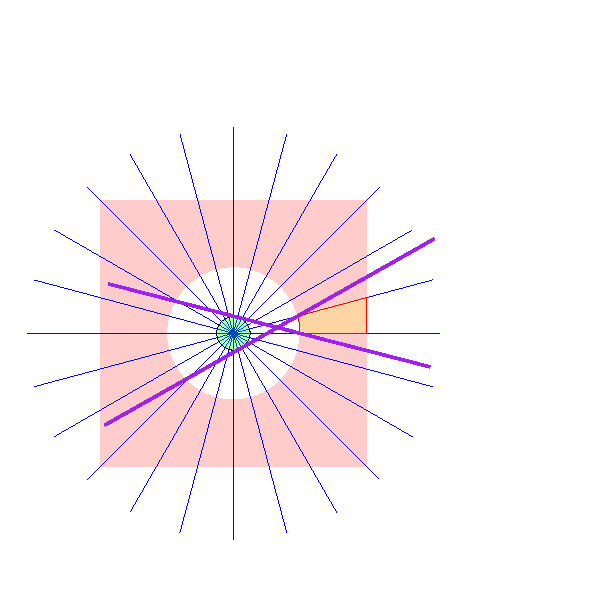
\includegraphics{figs/partition}}
    \caption{An illustration of refining the pairs in a \SSPD into pairs in opposite parts of an $\eps$-double-wedge. $\PSX$ is contained in the green square $\square$, while $\PSY$ is contained in the red square, and the white gap between them is a result of the separation property. The set of cones with the apex at the center of $\square$ give us the desired partition as demonstrated by the purple double-wedge. }
    \figlab{partition}
\end{figure}


\begin{lemma}
    \lemlab{refine:d:w}%
    %
    Given aמ $\eps^{-1}$-\SSPD $\WS$ of $n$ points in the plane, one
    can refine it, into aמ $\eps^{-1}$-\SSPD $\WS'$, such that each
    pair $\Pair = \{ \PSX, \PSY \} \in \WS'$ is contained in a
    $\eps$-double-wedge $\DW_\Pair$, such that $\PSX$ and $\PSY$ are
    contained in the two different faces of the double wedge
    $\DW_\Pair$. We have that $|\WS'| = O(|\WS|/\eps)$ and
    $\WeightX{\WS'} = O(\WeightX{\WS'}/\eps)$. The construction time
    is proportional to the weight of $\WS'$.
\end{lemma}
\begin{proof}
    By using \lemref{chop:easy}, we can assume that $\WS$ is (say)
    $(10/\eps)$-separated.  Now, the algorithm scans the pairs of
    $\WS$. For each pair $\Pair = \{ \PSX, \PSY \} \in \WS$, assume
    that $\diameterX{\PSX} < \diameterX{\PSY}$. Let $\square$ be the
    smallest axis-parallel square containing $\PSX$, centered at point
    $o$.  Partition the plane around $o$, by drawing around it
    $\Of(1/\eps)$ lines with the angle between any two consecutive lines
    being at most (say) $\eps/4$, see \figref{partition}. This
    partitions the plane into a set of cones $\ConeSet$. For a cone
    $C \in \ConeSet$, we show that there exists an $\eps$-double-wedge
    that contains $\PSX$ in one side, and $\PSY \cap C$ in the other.
    
    To see that, take the double-wedge formed by the cross tangents between  $\CHX{\PSX}$ and $\CHX{\PSY \cap C}$, where $\CHX{\PSX}$ denotes the convex-hull of $\PSX$. Assume w.l.o.g that $\square$ has side length 1, and let $c$ be a cone of angle $\eps / 4$ with apex $o$, whose angular bisector is a horizontal ray in the positive direction of the $x$ axis. See figure \figref{double-wedge} for an illustration.
    
    We would like to find a vertical segment $s$ such that all points of $Y$ lie to its right, with one endpoint on the upper line of $c$, and the other on the lower line of $c$. Using the segments' height and distance from the right side of $\square$ we will be able to get a bound on the angle of the cross tangents. We first find a segment $s$ with all points of $Y$ to its right. A trivial bound on that distance is given by the segment from, say, the lower left corner of $\square$, denoted $p$, of length $10/\eps$ with its right endpoint on the upper line of $c$, denote this point by $q$. This is due to the $10/\eps$ separation property of the SSPD. We know that this segment creates an angle of less than $\pi/4$ with the $x$-axis, since $o$ is the center of $\square$, and lies on the ray with apex $p$ that creates a $\pi/4$ angle with the $x$-axis. We therefore get that the $x$-coordinate difference between $\square$ and $q$ is at most $10/\eps\cdot \cos\frac{\pi}{4}-1\leq 7/\eps-1\leq 6/\eps$. So let $s'$ be a vertical segment between the upper and lower rays of $c$, with $x$-coordinate distance of $6/\eps-\frac{1}{2}$ from $\square$ (in order to make calculations easier). We get that $s'$ is of length $2\cdot \frac{6}{\eps}\tan \frac{\eps}{8}$. Finally, we take $s$ to be a vertical segment of length $\frac{12}{\eps}\tan \frac{\eps}{8}$, with its center on the $x$-axis at a distance of $5/\eps+\frac{1}{2}$ away from $o$. The angle of the $x$-axis and the segment between the lower end of the right side of $\square$ and the upper end of $s$ is now given by:
    
    \begin{equation*}
    	\arctan\left(\frac{\frac{6}{\eps}\tan\frac{\eps}{8}+\frac{1}{2}}{\frac{5}{\eps}}\right)%
    	=%
    	\arctan \left( \frac{6}{5}\tan\frac{\eps}{8}+\frac{\eps}{10} \right)%
    	=%
    	\Theta(\eps)%
    \end{equation*}

 
\end{proof}

\begin{figure}[h]
    \phantom{}\hfill%
    \includegraphics[page=2, width=0.48\linewidth]{figs/double_wedge}%
    \hfill%
    \includegraphics[page=3, width=0.48\linewidth]{figs/double_wedge}%
    \hfill%
    \phantom{}%
	\caption{An illustration of the proof for \lemref{refine:d:w}}
	\figlab{double-wedge}
\end{figure}


% -----------------------------------------------------------------------
\subsubsection{Delaunay triangulation}

We need the following well known property of Delaunay triangulation,
which would play a center role in our construction.

\begin{claim}
    \clmlab{d:t:connected}%
    %
    For a set of points $\PS \subseteq \Re^2$ in general position, let
    $\DT = \DTX{\PS}$ denote its Delaunay triangulation.  Then, for
    any closed disk $\disk$, we have $\restrictY{\DTX{\PS}}{\disk}$ is
    connected.
\end{claim}


\begin{proof}
    We first prove that for any (closed) disk $\disk$ with two points
    $\pa,\pb\in \PS$ on its boundary, there is a path between $\pa$
    and $\pb$ in $\restrictY{\DT}{\disk}$.  The proof is by induction
    over the number $m$ of points of $\PS$ in the interior of $\disk$:
    \begin{compactitem}
        \item $m=0$: The disk $\disk$ contains no points of $\PS$ in
        its interior, and thus $\pa \pb$ is an edge of the Delaunay
        triangulation, as $\disk$ testifies.

        \begin{figure}[h]
            \phantom{}\hfill%
            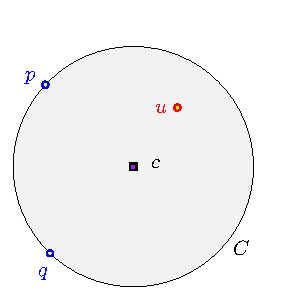
\includegraphics[page=1]{figs/shrink}%
            \hfill%
            \includegraphics[page=2]{figs/shrink}%
            \hfill%
            \includegraphics[page=3]{figs/shrink}%
            \hfill%
            \phantom{}%
            \caption{}
            \figlab{shrink}
        \end{figure}
        \item $m >0$: Let $\pc\in \PS$ be a point in the interior of
        $\disk$. We move the center $\cen$ of $\disk$ in the direction
        of $\pa$, shrinking $\disk$ in the process, so that the radius
        the disk is $\dY{\cen}{\pa}$, until we get a disk
        $\disk' \subseteq \disk$ such that $\pc$ is on the boundary of
        $\disk'$, see \figref{shrink}. Observe that $\pa$ and $\pc$
        are on the boundary of the new disk, and
        $|\interiorX{\disk'} \cap \PS| < |\interiorX{\disk} \cap
        \PS|$. Thus, by induction, there is a path $\gamma'$ between
        $\pa$ and $\pc$ in
        $\restrictY{\DT}{\disk'} \subseteq
        \restrictY{\DT}{\disk}$. Similarly, there must be a path
        $\gamma''$ between $\pc$ and $\pb$, and concatenating the two
        paths results in a path between $\pa$ and $\pb$ in
        $\restrictY{\DT}{\disk}$.
    \end{compactitem}
    \medskip%
    \noindent
    Back to the original claim.  For any two points
    $\pa,\pb \in \disk \cap \PS$ one can get a disk
    $\disk' \subseteq \disk$ that contains $\pa$ and $\pb$ on its
    boundary.  Indeed, shrink the radius of $\disk$ till, say, $\pa$
    is on the boundary, and then move the center of the disk towards
    $\pa$ while shrinking the size of the disk to maintain $\pa$ on
    the boundary, until $\pb$ is also on the boundary of the shrunken
    disk.
\end{proof}



%%%%%%%%%%%%%%%%%%%%%%%%%%%%%%%%%%%%%%%%%%%%%%%%%%%%%%%%%%%%%%%%%%%%%%%%%
\subsection{The construction of local spanners for disks}

\subsubsection{The construction}
\label{subsec:disk_construction}

The input is a set $\PS$ of $n$ points in the plane (in general
position) with $\spread = \spreadX{\PS}$, and a parameter
$\eps \in (0,1)$.

The algorithm computes a $1/\epsA$-\WSPD $\WS$ of $\PS$ using the
algorithm of \lemref{s:s:p:d:spread}, where $\epsA = \eps/6$.  For
each pair $\Pair = \{\PSX, \PSY \} \in \WS$, the algorithm computes
the Delaunay triangulation $\DT_{\Pair} = \DTX{ \PSX \cup \PSY}$. The
algorithm adds all the edges in $\DT_{\Pair} \cap (\PSX \otimes \PSY)$
to the computed graph $\G$.

\subsubsection{Analysis}

\paragraph{Size.}

For each pair $\Pair = \{\PSX, \PSY\}$ in the \WSPD, its Delaunay
triangulation contains at most $\Of( |\PSX| + |\PSY|)$ edges. As
such, the number of edges in the resulting graph is bounded by
\begin{equation*}
    \sum_{\{\PSX, \PSY\} \in \WS} O\bigl( |\PSX| + |\PSY| \bigr)
    =%
    O\pth{ \WeightX{\WS} }%
    =%
    O\pth{ \frac{n\log \spread}{{\epsA}^{2}}},
\end{equation*}
by \lemref{s:s:p:d:spread}.


\paragraph{Construction time.}
The construction time is bounded by
\begin{equation*}
    \sum_{\{\PSX, \PSY\} \in \WS} O\bigl( (|\PSX| + |\PSY|) \log
    (|\PSX| + |\PSY|)  \bigr)
    =%
    O\pth{ \WeightX{\WS} \log n }%
    =%
    O\pth{ \frac{n\log \spread \log n}{{\epsA}^{2}}},    
\end{equation*}

\paragraph{Local spanner property.}

\begin{lemma}
    Let $\G$ be the graph constructed above for the point set
    $\PS$. Then, for any (closed) disk $\disk$, and any two points
    $\px, \py \in \PS \cap \disk$, we have that
    $\restrictY{\G}{\disk}$ has a $(1+\eps)$-path between $\px$ and
    $\py$. That is, $\G$ is a $(1+\eps)$-local spanner for disks.
\end{lemma}

\begin{proof}
    The proof is by induction on the distance between $\pa$ and $\pb$
    (or more precisely, the rank of their distance among the
    $\binom{n}{2}$ pairwise distances).  Consider the pair
    $\Pair = \{ \PSX, \PSY \}$ such that $\px \in \PSX$ and
    $\py \in \PSY$.

    For the base case, consider the case that $\px$ is the
    nearest-neighbor to $\py$ in $\PS$, and $\py$ is the
    nearest-neighbor to $\px$ in $\PS$.  It must be, because of the
    separation property of $\Pair$, that $\PSX$ and $\PSY$ are
    singletons. Indeed, if $\PSX$ contains another point, then $\py$
    would not be the nearest-neighbor to $\px$ (this is true for
    $\epsA < 0.5$). As such, $\px \py \in \DT_\Pair$,
    $\px, \py \in \disk$, and the edge $\px \py \in \EGX{\G}$,
    implying the claim.

    For the inductive step, observe that the claim follows if
    $\px \py \in \DT_\Pair$, so assume this is not the case. By the
    connectivity of $\DT_\Pair \cap \disk$, see
    \clmref{d:t:connected}, there must be points
    $\px' \in \PSX \cap \disk$, $\py' \in \PSY \cap \disk$, such that
    $\px'\py' \in \EGX{ \DT_\Pair}$. As such, by construction, we have
    that $\px'\py' \in \EGX{\G}$. Furthermore, by the separation
    property, we have that
    \begin{equation*}
        \max \pth{ \diameterX{\PSX}, \diameterX{\PSY} }%
        \leq%
        \epsA \cdot \dsY{\PSX}{\PSY}%
        \leq%
        \epsA \ell, 
    \end{equation*}
    where $\ell = \dY{\px}{\py}$. In particular,
    $\dY{\px'}{\px} \leq \epsA \ell$ and
    $\dY{\py'}{\py} \leq \epsA \ell$. As such, by induction, we have
    $\dGZ{\G}{\px}{\px'} \leq (1+\eps)\dY{\px}{\px'} \leq
    (1+\eps)\epsA \ell$ and
    $\dGZ{\G}{\py}{\py'} \leq (1+\eps)\dY{\py}{\py'} \leq
    (1+\eps)\epsA \ell$.  Furthermore,
    $\dY{\px'}{\py'} \leq (1+2\epsA)\ell$. As $\px'\py' \in \EGX{\G}$,
    we have
    \begin{align*}
      \dGZ{\G}{\px}{\py}%
      &\leq%
        \dGZ{\G}{\px}{\px'}%
        +\dY{\px'}{\py'}
        +
        \dGZ{\G}{\py'}{\py}%
        \leq%
        (1+\eps)\epsA \ell
        +(1+2\epsA)\ell
        + (1+\eps)\epsA \ell
        \leq%
        \pth{ 2\epsA +1+2\epsA + 2\epsA } \ell        
      \\&%
      =%
      \pth{ 1+ 6\epsA  } \ell        
      \leq%
      \pth{ 1+ \eps  } \dY{\px}{\py},
    \end{align*}
    if $\epsA \leq \eps/6$.
\end{proof}

\paragraph{The result.}

\begin{theorem}
    \thmlab{main:1}%
    %
    Let $\PS$ be a set of $n$ points in the plane, and let
    $\eps \in (0,1)$ be a parameter. The above algorithm constructs a
    local $(1+\eps)$-spanner $\G$ for disks. The spanner has
    $\Of\pth{ \eps^{-2} n\log \spread }$ edges, and the construction time
    is $\Of\pth{ \eps^{-2} n\log \spread \log n }$.  Formally, for any disk
    $\disk$ in the plane, and any two points
    $\pa, \pb \in \PS \cap \disk$, we have a $(1+\eps)$-path in
    $\restrictY{\G}{\disk}$.
\end{theorem}

% ------------------------------------------------------------------------
\subsubsection{Applications and comments}


\begin{defn}
    Given a region $R$ in the plane and a point set $\PS$, consider
    two points $\pa, \pb \in \PS$. The edge $\pa \pb$ is \emphw{safe}
    in $R$, if there is a disk $\disk$ such that
    $\pa,\pb \in \disk \subseteq R$. Let $\GY{\PS}{R}$ be the graph
    formed by all the safe edges in $\PS$ for $R$. Note, that this
    graph might have a quadratic number of edges in the worst case.
\end{defn}

Observe that $\GY{\Re^2}{\PS}$ is a clique.

\begin{corollary}
    Let $\PS$ be a set of $n$ points in the plane, and let
    $\eps \in (0,1)$ be a parameter, and let $\G$ be a local
    $(1+\eps)$-spanner of $\PS$ for disks. Then, for a region $R$ in the
    plane, if we denote the graph $\GA = \GY{\PS}{R}$, we have that
    $\restrictY{\G}{R}$ is a $(1+\eps)$-spanner for
    $\restrictY{\GA}{R}$. Formally, for any two points
    $\pa, \pb \in \PS \cap R$, we have that
    $\dGZ{\GA}{\pa}{\pb} \leq (1+\eps)\dGZ{\G}{\pa}{\pb}$.

    In particular, for any convex region $C$, the graph $\G \gminus C$
    is a $(1+\eps)$-spanner for $\GY{\Re^2}{\PS} \gminus C$.
\end{corollary}
\begin{proof}
    Consider the shortest path $\pi = u_1 u_2 \ldots u_k$ between
    $\pa$ and $\pb$ in $\dGZ{\GA}{\pa}{\pb}$. Every edge
    $e_i = u_i u_{i+1}$ has a disk $\disk_i$ such that
    $u_i, u_{i+1} \in \disk_i \subseteq R$. As such, there is a
    $(1+\eps)$-path between $u_i$ and $u_{i+1}$ in
    $\restrictY{\G}{\disk_i} \subseteq
    \restrictY{\G}{R}$. Concatenating these paths directly yields the
    desired result.

    The second claim follows by observing that the complement of $C$
    is the union of halfspaces, and halfspaces can be considered to be
    ``infinite'' radius disks. As such, the above argument applies
    verbatim.
\end{proof}

\paragraph{But why not \SSPD?}

The result of \thmref{main:1} is somewhat disappointing as it depends
on the spread of the point set (logarithmically, but still). A natural
way is to try and emulate the construction of Abam \etal
\cite{abfg-rftgs-09} and use a \SSPD instead of a \WSPD. The total weight
of the \SSPD is near linear (with no dependency on the
spread). Furthermore, after some post processing, one can assume every
pair $\Pair = \{ \PSX, \PSY \}$ is angularly $\eps$-separated -- that
is, there is a double wedge with angle $\leq \eps$, such that $\PSX$
and $\PSY$ are of different sides of the double wedge. The problem is
that for the local disk $\disk$, it might be that the bridge edge between
$\PSX$ and $\PSY$ that is in $\DT_\Pair \cap \disk$ is much longer
than the distance between the two points of interest. This somewhat counter-intuitive
situation is illustrated in \figref{bad}.

\begin{figure}[h]
    \phantom{} \hfill%
    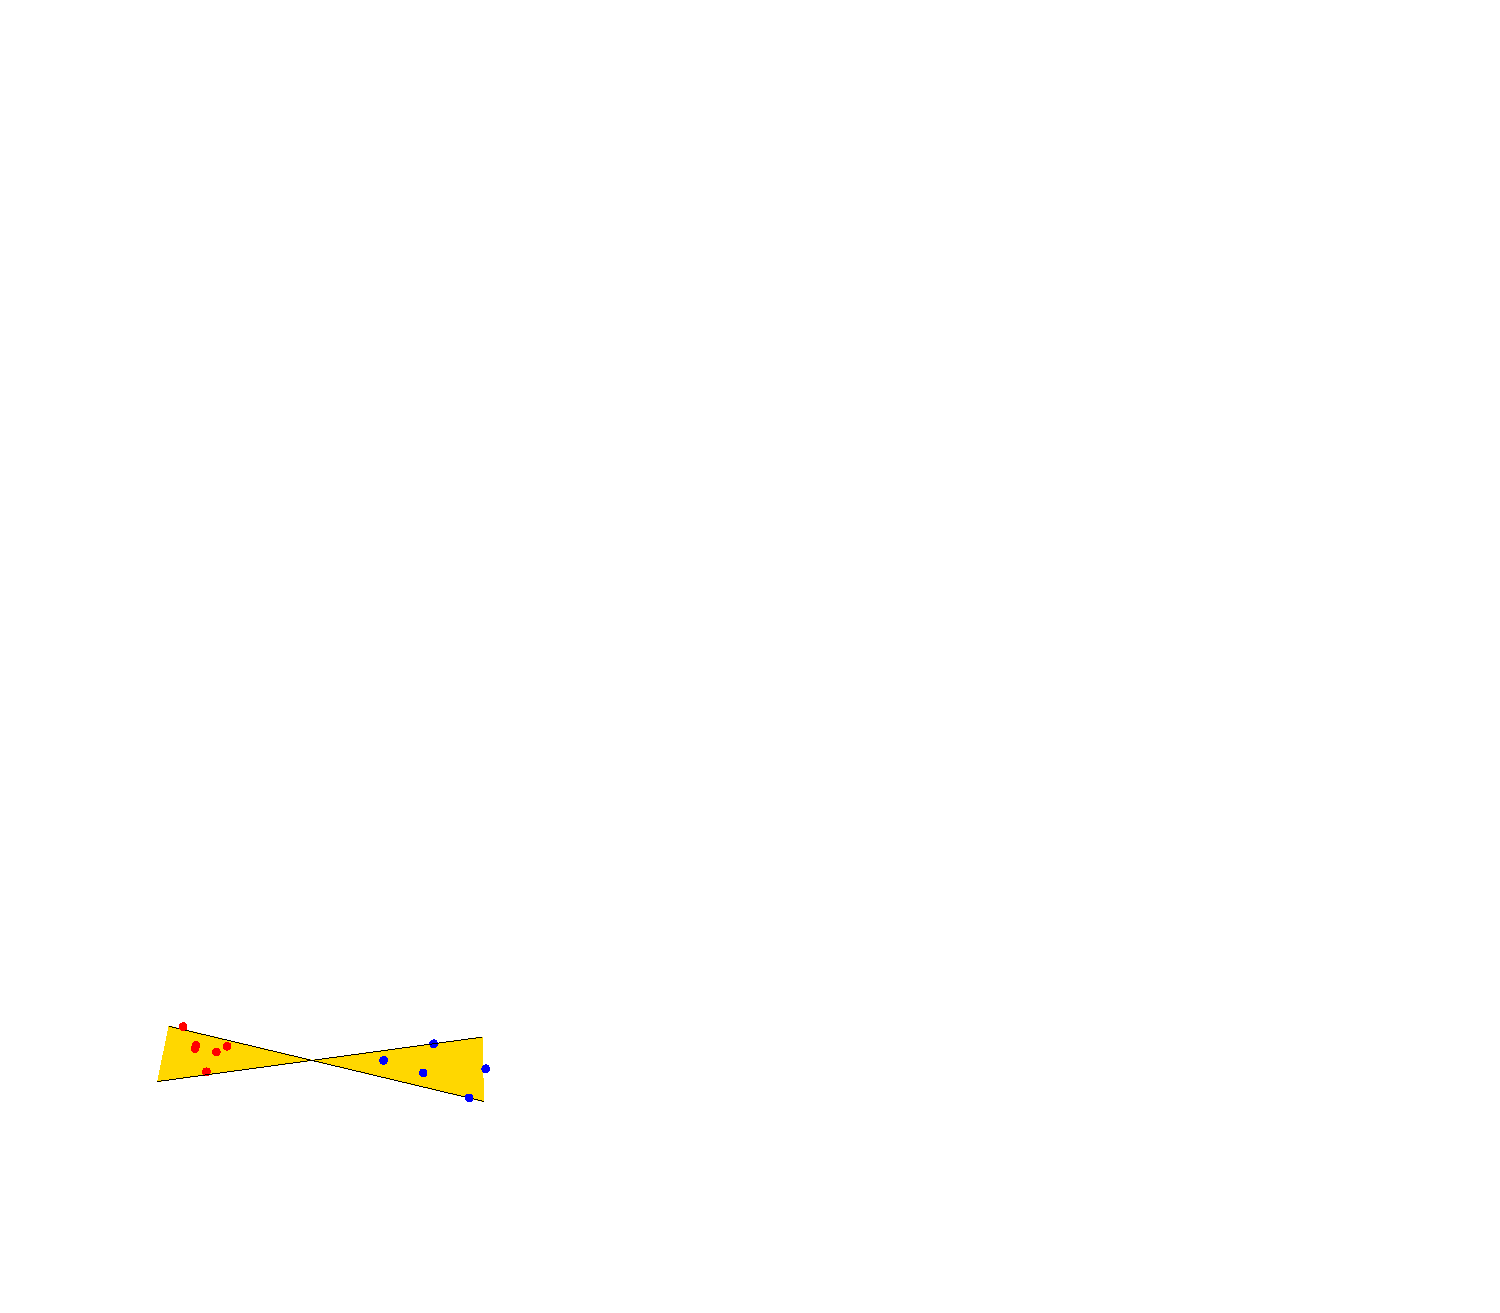
\includegraphics[page=1]{figs/bad_example} \hfill%
    \includegraphics[page=2]{figs/bad_example} \hfill%
    \includegraphics[page=3]{figs/bad_example} \hfill%
    \phantom{}
    \caption{A bridge too far -- the only surviving bridge between the
       red and blue points is too far to be useful if the sets of
       points are not well separated.}
    \figlab{bad}
\end{figure}


% ~\newpage ~\newpage ~\newpage

%%%%%%%%%%%%%%%%%%%%%%%%%%%%%%%%%%%%%%%%%%%%%%%%%%%%%%%%%%%%%%%%%%%%%%%%%
\subsubsection{A lower bound for local spanner for disks}

\begin{figure}[h]
    \centering%
    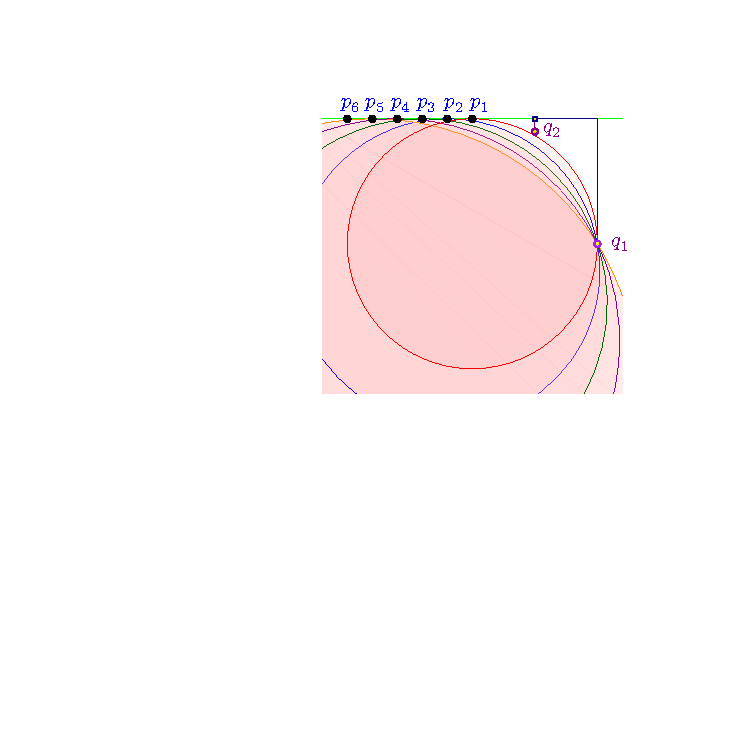
\includegraphics{figs/lower_bound}%
    \caption{The set of disks $D_1$, and the construction of $\pb_2$.}
    \figlab{flower}
\end{figure}

\begin{lemma}
    \lemlab{l:s:lower:bound}%
    %
    For $\eps =1/4$, and parameters $n$ and $\spread \geq 1$, there is
    a point set $\PS$ of $n + \ceil{\log \spread}$ points in the
    plane, with spread $O( n \spread )$, such that any local
    $(1+\eps)$-spanner of $\PS$ for disks, must have
    $\Omega( n \log \spread )$ edges.
\end{lemma}


\begin{proof}
    Let $\pa_i = (-i, 0)$, for $i=1, \ldots, n$.  Let
    $M = 1+ \ceil{ \log_2 \spread }$ and $\pb_1 = (n 2^M, -1)$.  For a
    point $\pa$ on the $x$-axis, and a point $\pb$ below the $x$-axis, and
    to the right of $\pa$, let $\diskVY{\pa}{\pb}$ be the disk whose
    boundary passes through $\pa$ and $\pb$, and its center has the
    same $x$-coordinate as $\pa$.
    
    In the $j$\th iteration, for $j=2,\ldots, M-1$, Let $x_j = n2^{M-j+1} = x(\pb_{j-1})/2$, and
    let $y_j < 0$ be the maximum $y$-coordinate of a point that lies
    on the intersection of the vertical line $x =x_j$ and the disks of
    $D_1 \cup \cdots \cup D_j$. Let $\pb_j = (x_j, 0.99
    y_j)$. Consider the set
    of disks
    \begin{equation*}
        D_j = \Set{ \diskVY{\pa_i}{\pb_{j-1}} }{i=1,\ldots, n},
    \end{equation*}
    see \figref{flower}.
    
 	Clearly, the point $\pb_j$ lies outside all the disks of
    $D_1 \cup \ldots \cup D_j$. The construction now continues to the
    next value of $j$. Let
    $\PS = \{ \pa_1, \ldots, \pa_n, \pb_2, \ldots, \pb_M \}$. We have
    that $|\PS| = n + M-1$.

    The minimum distance between any points in the construction is $1$
    (i.e., $\dY{\pa_1}{\pa_2}\bigr.$). Indeed $x(\pb_M) = 2n$ and thus
    $\dY{\pb_M}{\pa_1} \geq 2n$.  The diameter of $\PS$ is
    $\dY{\pa_1}{\pb_1} = \sqrt{(n +n2^{M})^2+ 1} \leq 2 n 2^M $. As
    such, the spread of $\PS$ is bounded by
    $\leq n 2^{M+1} = O( n \spread)$.

    For any $i$ and $j$, consider the disk
    $\diskVY{\pa_i}{\pb_j}$. This disk does not contain any point of
    $\pa_1,\ldots, \pa_{i-1}, \pa_{i+1}, \ldots, \pa_{n}$ since its
    interior lies below the $x$-axis. By construction it does not
    contain any point $\pb_{j+1}, \ldots, \pb_{M-1}$. This disk
    potentially contains the points $\pb_{j-1}, \ldots, \pb_1$,
    but observe that for any index $k \in \IRX{j-1}$, we have that
    \begin{equation*}
        \dY{\pa_i}{\pb_k} %
        =%
        \sqrt{ \pth{i + n 2^{M-k+1} }^2 + \bigl( y(\pb_j) \bigr)^2 },
    \end{equation*}
    which implies that
    \begin{math}
        n 2^{M-k+1}%
        \leq%
        \dY{\pa_i}{\pb_k} %
        <%
        n( 2^{M-k+1} +2).
    \end{math}
    We thus have that
    \begin{equation*}
        \frac{\dY{\pa_i}{\pb_k}}{\dY{\pa_i}{\pb_j}}
        \geq%
        \frac{n 2^{M-k+1}}{n( 2^{M-j+1} +2)}
        =%
        \frac{ 2^{M-j}\cdot 2^{j-k}}{ 2^{M-j} +1}
        =%
        \frac{  2^{j-k}}{ 1 + 1/2^{M-j}}
        \geq
        \frac{2}{1+1/2}
        = \frac{4}{3}
        > 1+\eps,
    \end{equation*}
    since $j \in \IRX{M-1}$.  Namely, the shortest path in $\G$
    between $\pa_i$ and $\pb_j$, can not use any of the points
    $\pb_{1}, \ldots \pb_{j-1}$. As such, the graph $\G$ must contain
    the edge $\pa_i \pb_j$. This implies that
    $|\EGX{\G}| \geq n (M-1)$, which implies the claim.
\end{proof}



%%%%%%%%%%%%%%%%%%%%%%%%%%%%%%%%%%%%%%%%%%%%%%%%%%%%%%%%%%%%%%%%%%%%%%%%% 
%%%%%%%%%%%%%%%%%%%%%%%%%%%%%%%%%%%%%%%%%%%%%%%%%%%%%%%%%%%%%%%%%%%%%%%%%
%%%%%%%%%%%%%%%%%%%%%%%%%%%%%%%%%%%%%%%%%%%%%%%%%%%%%%%%%%%%%%%%%%%%%%%%%



\subsection{Homothets of a convex region}
\label{subsection:homothets}

Using arguments similar to those used for disk local spanners, we now extend the results for the case where
$\FF$ is the set of all scaled and translated copies of a
convex shape $\CC$. This family of regions is also known as homothets of $\CC$. Formally, the homothet of the shape $\CC$ with center $o$ and scaling $\lambda$ is the set $\{o + \lambda o \pa : \pa \in \CC\}$. See \figref{homothet}. While the Delaunay triangulation is not well
defined for all convex shapes, the operation of creating edges between every
two points $\pa,\pb\in \PS$ such that there exist a homothet of $\CC$ that
contains only $\pa$ and $\pb$ and no other point of $\PS$, is well
defined for a point set in general position, and gives us a graph known as the $\CC$-Delaunay graph of $\PS$. We denote the $\CC$-Delaunay graph of $\PS$ by $\DG_{\CC}(\PS)$. 
Note that in these settings, the meaning of general position is that no 3 points of $\PS$ lie on the boundary of a homothet of $\CC$.


\begin{figure}[h]
	\centering%
	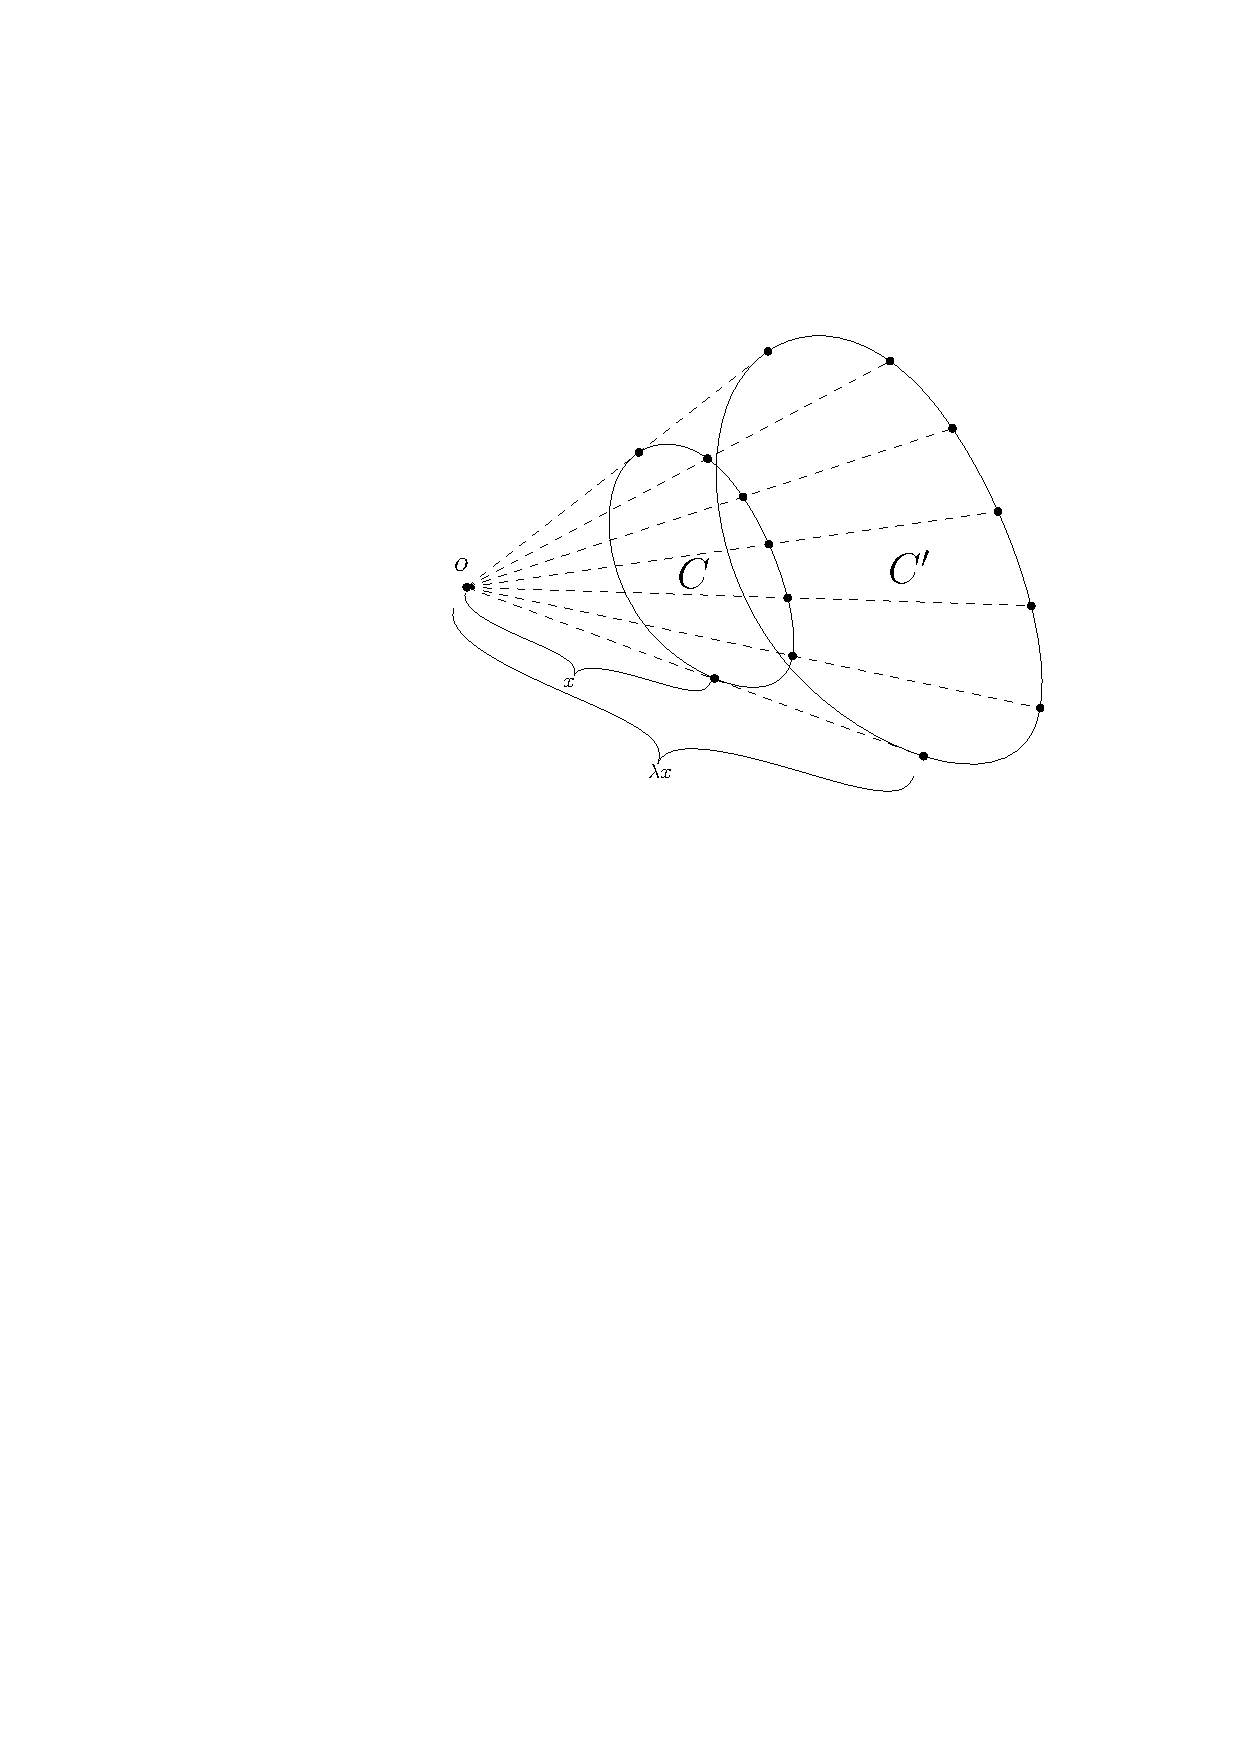
\includegraphics{figs/homothet}%
	\caption{$C'$ is a homothet of $C$ of center $o$ and scaling $\lambda$.}
	\figlab{homothet}
\end{figure}


\begin{claim}
	\clmlab{c:t:connected}%
	%
	Given a set of points $\PS \subseteq \Re^2$ in general position, and a convex shape $\CC$, let $\DG = \DG_{\CC}(\PS)$ denote the $\CC$-Delaunay graph of $\PS$. For any homothet $C$ of $\CC$, we have $\restrictY{\DG}{C}$ is connected.

\end{claim}


\begin{proof}
	This proof very closely resembles that of \clmref{d:t:connected}. The second part of both claims is actually identical, and we therefore only prove that  for any (closed) convex region $\CC$ with two points $\pa,\pb\in \PS$ on its boundary, there is a path between $\pa$ and $\pb$ in $\restrictY{\DG}{C}$.
	The proof is again by induction over the number of points of $\PS$ in the interior of $C$, and is very similar to its counterpart in \clmref{d:t:connected}. The only difference here is that shrinking an arbitrary convex region towards a point on the boundary is not well defined.
	Luckily, it is not hard to prove that such a procedure is possible, and after proving this, the rest of the proof is exactly as that of \clmref{d:t:connected}.
	So, let  $C$ be a homothet of $\CC$ such that $\pa\in\PS\cap\partial C$. We define shrinking $C$ by a factor of $\lambda$ towards $\pa$ as a homothetical translation of $C$ with center $\pa$ and scaling factor $\lambda$. Since $C$ is convex we have that the resulted region $C'$ is contained in $C$, and by the definition of a homothet we have that $C'$ is a homothet of $C$.
	This finishes the proof since we can now follow the proof of \clmref{d:t:connected}.

\end{proof}

Notice that for any convex region $\CC\subseteq \Re^2$ and two points $\pa,\pb \in C$, there exists a homothet $C$ of $\CC$ with $\pa$ and $\pb$ on its boundary, and such that $C\subseteq \CC$. This can be seen in much the same way that a similar claim is proven for disks, as we can shrink $\CC$ towards the center of the segment $\overline{\pa\pb}$ until one of the points lie on the boundary of the shape, and then shrink it further toward that point, which now lies on the boundary, until the second point is on the boundary as well. Since the center of the shrinking process are always contained in the shrinking convex shape, we get that at it is always inside the its unshrinked version.

%\begin{claim}
%	\clmlab{c:t:planar}%
%	%
%	Given a set of points $\PS \subseteq \Re^2$ in general position, and a convex shape $\CC$. $\DG_{\CC}(\PS)$, the $\CC$-Delaunay graph of $\PS$, is planar.
%	
%\end{claim}
%
%
%\begin{proof}
%	Let $e=\overline{\pa\pb}, e'=\overline{\pa'\pb'}$ be two edges of $\DG_{\CC}(\PS)$, and assume for a contradiction that $e$ intersects $e'$. W.l.o.g, we assume that $e$ is horizontal, $\pa'$ is above the line $l$ containing $e$, and $\pb'$ is below it.
%	
%	Let $C$ be a homothet of $\CC$ containing $\pa$ and $\pb$ on its boundary, and that contains no other point of $\PS$. Such a homothet exists since $\CC$ is convex, and $e\in \DG_{\CC}(\PS)$.  Let $\phi : [0,1] \longrightarrow C$ be a parameterization of $C$ such that $\phi(x_\pa)=\pa$, and $\phi(x_\pb)=\pb$. Similarly, let $C'$ be a homothet of $\CC$ containing $\pa'$ and $\pb'$ on its boundary, and that contains no other point of $\PS$ and let $\psi(x):= c + \alpha x$ be the translation and scaling such that $\psi(C) = C'$.
%	
%	We denote the segment $\overline{\psi(\phi(x_\pb))\psi(\phi'(x_\pb))}$ by $s$. This is a segment contained in $C'$ that corresponds to $e$ in $C$, meaning that it is horizontal, and has both endpoints on the boundary of $C'$. W.l.o.g, we assume that $s$ lies above $l$. The convex hull of $s\cup \pb$ is triangle $\Delta'$ that is contained in $C'$. We claim that $\psi^{-1}(\Delta')=\Delta$ is contained in $C$, and contains $\pb$, thus contradicting the choice of $e$. First, $\Delta\subseteq C$ by the definition of $\psi$. We now notice that the two non-horizontal edges of $\Delta'$ intersect $e$, since otherwise we would have that either $\pa$ or $\pb$ are contained in $C'$, contradicting the choice of $e'$. Now, since $\Delta \approx \Delta'$ we have that the part of $\Delta'$ below $l$ is contained in $\Delta$, and we are thus done. See \figref{planar_DG} for an illustration.
%	
%\end{proof}
%
%\begin{figure}[h]
%	\centering%
%	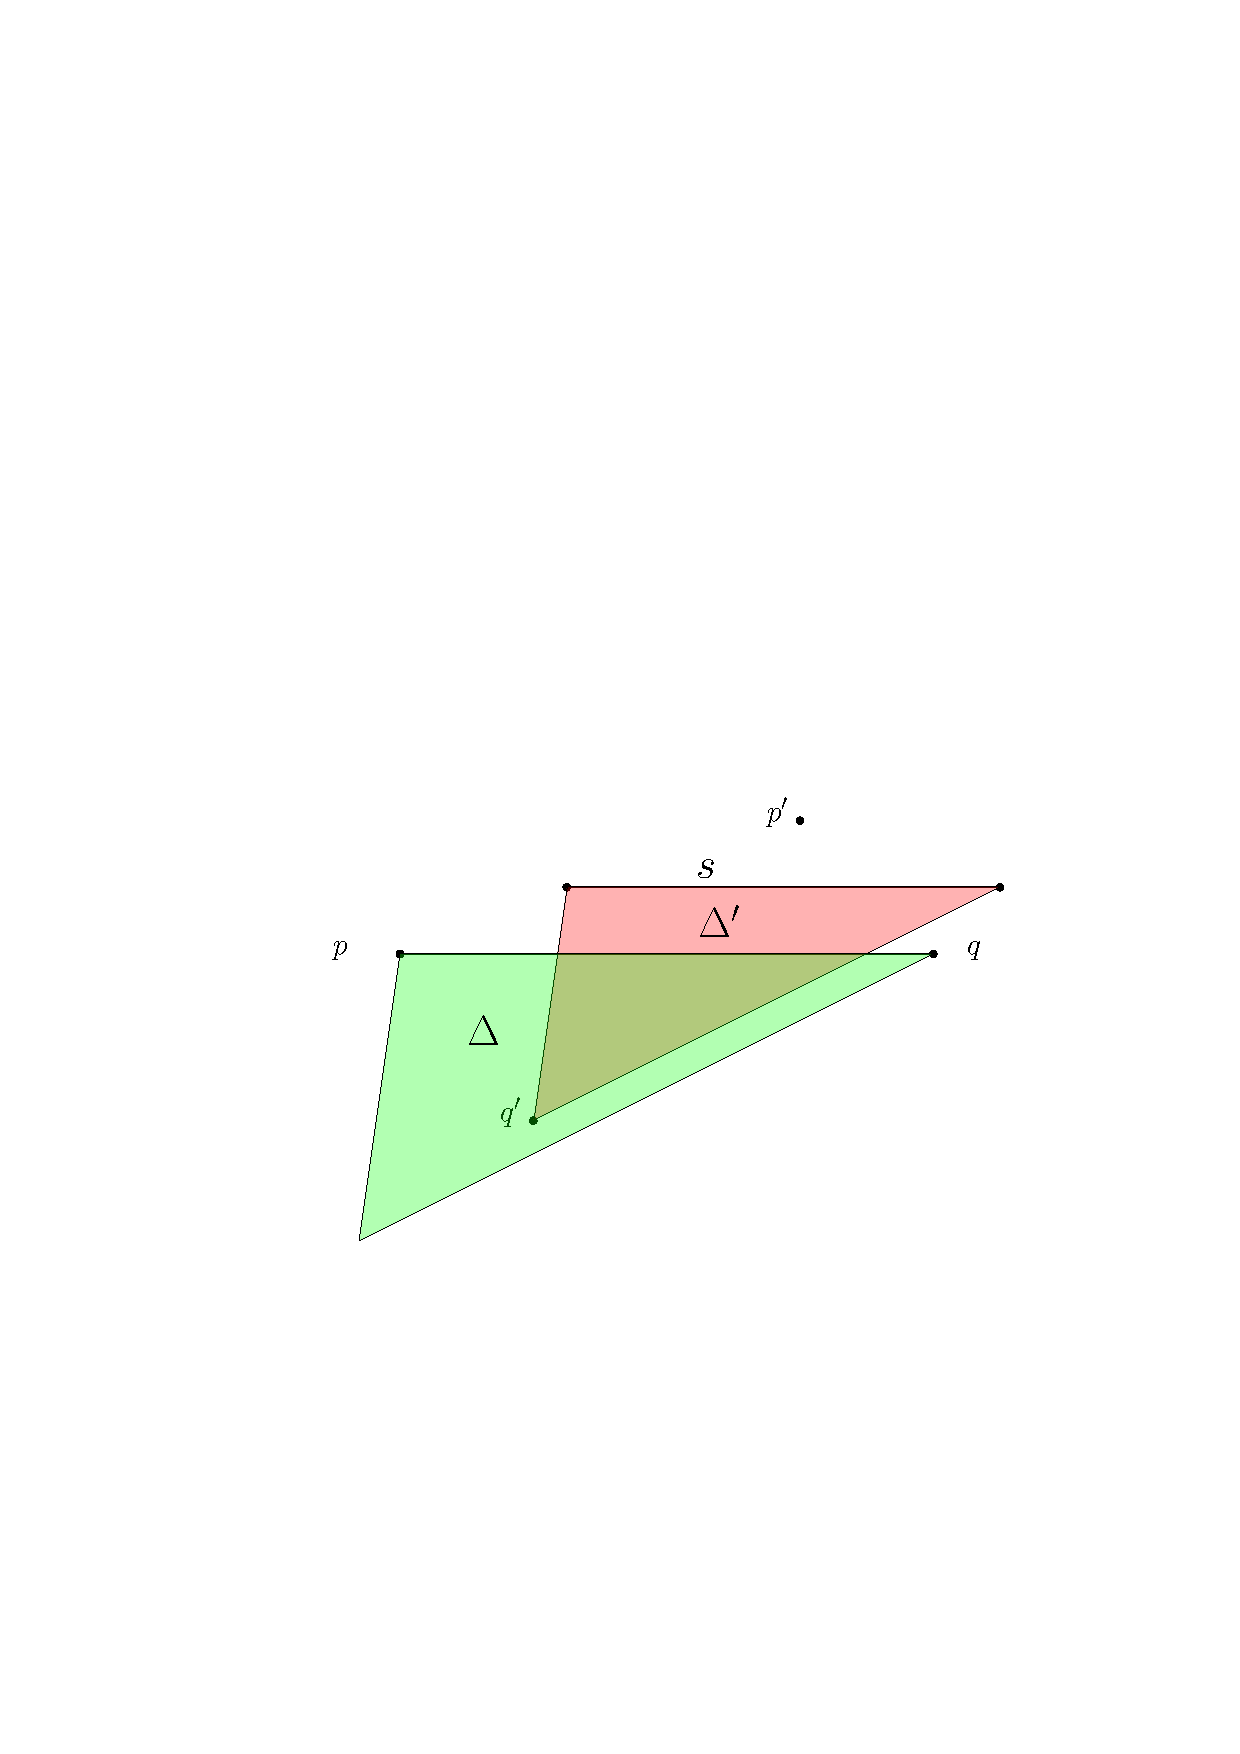
\includegraphics[]{figs/planar_DG}%
%	\caption{An illustration of the proof of the planarity of the $\CC$-Delauny graph }
%	\figlab{planar_DG}
%\end{figure}

We will need the following from the paper of Chew and Drysdale~\cite{cd-vdbcdf-85} in order to construct the spanner, and bound its size similarly to the local disk spanner.  

\begin{theorem}[\cite{cd-vdbcdf-85}]
	\thmlab{c:t:construct_delaunay_graph}%
	For any convex shape $\CC$ and a set of points $\PS$, $\DG_{\CC}(\PS)$ can be computed in $O(n \log n)$ time.
\end{theorem}

\begin{lemma}[\cite{cd-vdbcdf-85}]
	\lemlab{c:t:linear_size}%
	For any convex shape $\CC$ and a set of points $\PS$, $\DG_{\CC}(\PS)$ has $O(n)$ edges, vertices, and faces.
\end{lemma}


\paragraph{The result}
\begin{theorem}
	\thmlab{l:s:homothets}
	%
	Let $\PS$ be a set of $n$ points in the plane, and let
	$\eps \in (0,1)$ be a parameter. We can constructs a
	local $(1+\eps)$-spanner $\G$ for homothets of a convex region $\CC$. The spanner has $\Of\pth{ \eps^{-2} n\log \spread }$ edges, and the construction time
	is $\Of\pth{ \eps^{-2} n\log \spread \log n }$.  Formally, for any homothet $C$ of the convex region
	$\CC\subseteq \Re^2$, and any two points
	$\pa, \pb \in \PS \cap \disk$, we have a $(1+\eps)$-path in
	$\restrictY{\G}{C}$.
\end{theorem}

\begin{proof}
	Due to \thmref{c:t:construct_delaunay_graph}, \lemref{c:t:linear_size}, and \clmref{c:t:connected}, we can use the algorithm in subsection \ref{subsec:disk_construction} verbatim, switching only the conventional Delaunay triangulation with the $\CC$-Delaunay graph. Since the $\CC$-Delaunay graph has linear complexity for any convex shape $\CC$ the size of the spanner can be bounded using the same asymptotic bounds as the disk local spanner, and since the $\CC$-Delaunay graph can be constructed in $O(n\log n)$ time, the time complexity bounds hold as well. The correctness proof of \thmref{main:1} uses only the connectivity of the Delaunay triangulation, and thus the same proof suffices.
	

\end{proof}



%%%%%%%%%%%%%%%%%%%%%%%%%%%%%%%%%%%%%%%%%%%%%%%%%%%%%%%%%%%%%%%%%%%%%%%%% 
%%%%%%%%%%%%%%%%%%%%%%%%%%%%%%%%%%%%%%%%%%%%%%%%%%%%%%%%%%%%%%%%%%%%%%%%%
%%%%%%%%%%%%%%%%%%%%%%%%%%%%%%%%%%%%%%%%%%%%%%%%%%%%%%%%%%%%%%%%%%%%%%%%%



\section{A local spanner for axis parallel squares}
\seclab{squares}
One can modify the above construction for axis-parallel squares, and
get a local spanner without dependency on the spread.

\subsubsection{Construction}

The input is a point set $\PS$ of $n$ points in the plane, and an
approximation parameter $\eps \in (0,1/2)$.  We assume that the input
point set $\PS$ is in general position. Specifically, no two points of
$\PS$ share a coordinate value, or appear in opposing corners of an
axis-parallel square -- this can be ensured by slightly perturbing the
points if necessary. %TODO: IS THIS LEGAL IN THIS CASE?


One can define the Delaunay triangulation when the unit ball is
replaced by the unit square. Formally, in this triangulation two
points are connected $\iff$ there is a square that contains these two
points on its boundary and no points in its interior. Let
$\DT_\square$ denote the resulting \emphw{$L_\infty$-Delaunay
   triangulation}.

Let $\epsA = \eps/20$.  Instead of constructing a \WSPD, the algorithm
computes a $1/\epsA$-\SSPD $\WS$, using the algorithm of
\thmref{S:S:P:D:main}. By using the algorithm of \lemref{refine:d:w}, and increasing the weight and number of pairs by a
factor of $\Of(1/\epsA)$,
one can assume that every pair $\{ \PSX, \PSY \} \in \WS$ is not only
semi-separated, but also that there is an associated double wedge of angle
$\leq \epsA$ containing $\PSX$ and $\PSY$ in opposing wedges.  The algorithm now computes the ``square'' Delaunay
triangulation for each such pair, and adds the edges of the
triangulation to the resulting graph $\G$.



\subsubsection{Analysis}

\paragraph{Size and running time.}

Computing the \SSPD takes $\Of\pth{n \epsA^{-2} \log n}$ time, and the
refinement takes $\Of\pth{n \epsA^{-3} \log n}$ time (which is also the
weight of the resulting \SSPD). The number of edges of each
$L_\infty$-Delaunay triangulation for a pair is proportional to its
weight, which implies that the total number of edges in the resulting
graph $\G$ is $\Of\pth{ \epsA^{-3} n\log n}$. Computing all these
Delaunay triangulations takes $\Of\pth{ \epsA^{-3}n \log^2 n}$ time.


\paragraph{Shrinking squares.}
We need the following lemma about the shrinking of axis-parallel squares.
Observe that this property definitely does not hold for disks, as
illustrated in \figref{bad}.

\begin{lemma}
    \lemlab{shrink:squars}%
    %
    (A) Let $\sqr$ be an axis parallel square in the plane, and let
    $\pa, \pb$ be two arbitrary points in $\sqr$. Then, there is a
    square $\sqrA \subseteq \sqr$ that contains $\pa$ and $\pb$ on its
    boundary.

    (B) Let $\sqr$ be as before, and let $\PSX, \PSY$ be two point sets in the plane, such that
    $\PSX' = \PSX \cap \sqr \neq \emptyset$ and
    $\PSY' = \PSY \cap \sqr \neq \emptyset$. Let
    $\px \in \PSX, \py \in \PSY$ be the two points realizing
    $\dsZ{\infty}{\PSX'}{\PSY'} = \underset{\pa \in \PSX', \pb \in \PSY'}{\min}
    \dZ{\infty}{\pa}{\pb}$. Then, there is a square
    $\sqrA \subseteq \sqr$ that contains $\px$ and $\py$ on its
    boundary, and $\sqrA$ does not contain any other point of
    $\PSX \cup \PSY$.
\end{lemma}
\begin{proof}
    (A) Start shrinking $\sqr$ around its center till it contains one
    of the points (say $\pa$ is on its boundary. Next, move the center
    of the square towards $\pa$ till the boundary of the continuously
    shrinking square passes through $\pb$. If $\pa$ and $\pb$ lie on
    adjacent edges, then continue the shrinking process by moving the
    center towards the common corner of the shared edges -- this
    process stops when one of the points is on the corner of the
    square.  Clearly, the resulting square $\sqrA$ is the desired
    square, see \figref{shrink:sq}.

    \begin{figure}[h]
        \phantom{}\hfill%
        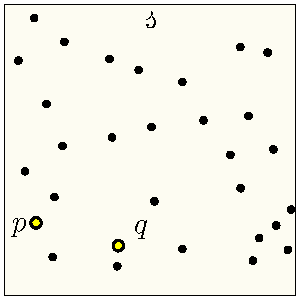
\includegraphics[page=1,width=0.2\linewidth]{figs/shrink_sq}
        \hfill%
        \includegraphics[page=2,width=0.2\linewidth]{figs/shrink_sq}%
        \hfill%
        \includegraphics[page=3,width=0.2\linewidth]{figs/shrink_sq}%
        \hfill%
        \includegraphics[page=4,width=0.2\linewidth]{figs/shrink_sq}
        \hfill\phantom{}%

        \caption{}
        \figlab{shrink:sq}
    \end{figure}

    (B) Let $r = \dsZ{\infty}{\PSX'}{\PSY'}$. By (A), there is a
    square $\sqrA \subseteq \sqr$ having $\px$ and $\py$ on apposing
    sides. As such, the side length of $\sqrA$ is $r$. Assume for
    contradiction, that there is some other point
    $\px' \in \PSX \cap \sqrA$. By our general position assumption,
    $\px'$ is in the interior of $\sqrA$, and in particular,
    $\dZ{\infty}{\px'}{\py} < r$, which is a contradiction to the
    choice of $\px$ and $\py$.
\end{proof}

\paragraph{Local spanner property.}
\begin{lemma}
    \lemlab{squares}%
    %
    For any axis parallel square $\sqr$ in the plane, and any two
    points $\pa, \pb \in \PS \cap \sqr$, we have a $(1+\eps)$-path in
    $\restrictY{\G}{\sqr}$.
\end{lemma}
\begin{proof}
    We prove the existence of a $(1+\eps)$-path between every pair $x,y\in  \PS \cap \sqr$ of points, by induction over the rank of $\dY{\px}{\py}$. The base case is simple, as the pair $(\{\px\},\{\py\})$ is a pair in $\WS$, and $xy$ is thus an edge in $G$. Now, consider two points $\px, \py \in \PS \cap \sqr$, where $\sqr$ is
    some arbitrary square. There exists a pair
    $\Pair = \{ \PSX, \PSY \} \in \WS$ such that $\px \in \PSX$ and
    $\py \in \PSY$, and this pair is $\epsA^{-1}$-semi separated and
    is also separated by a double wedge of angle $\leq \epsA$.  See
    \figref{infty:spanner}.  Furthermore, assume that
    $\diameterX{\PSX} < \diameterX{\PSY}$.
 
    \begin{figure}[h]
        \hfill%
        {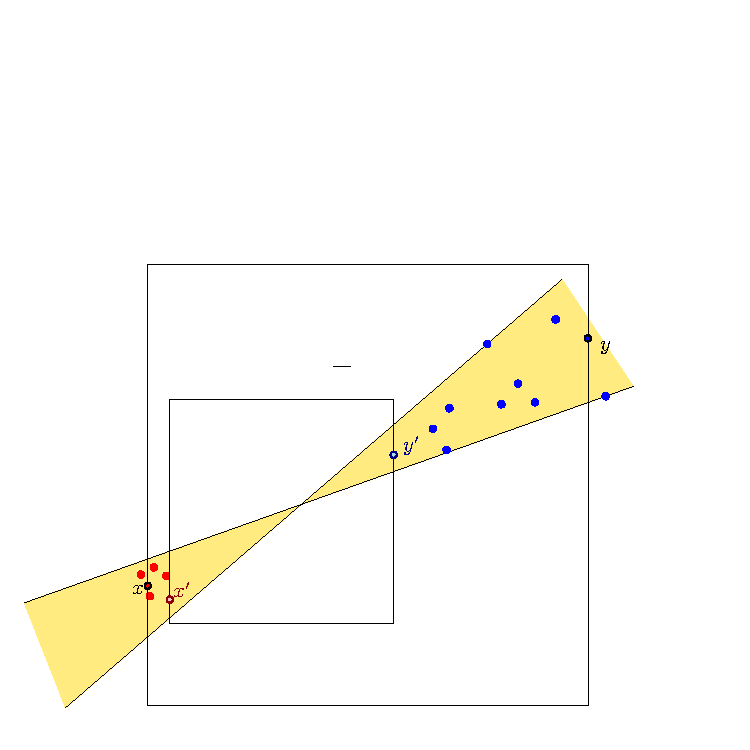
\includegraphics{figs/spanner_sq}} \hfill%
        \phantom{}%
        % 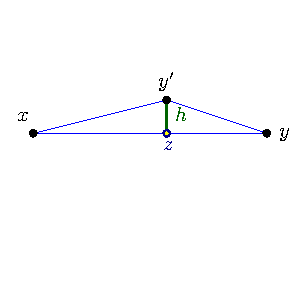
\includegraphics{figs/triangle}%
        \caption{A square region $\sqrA$ and two double-wedge semi-separated point sets $\PSX$ (red) and $\PSY$ (blue. Notice that while $\px'$ and $\py'$ are the closest pair using $L_\infty$, that is not necessarily true for the Euclidean distance.}
        \figlab{infty:spanner}
    \end{figure}

    Let $\PSX' = \PSX \cap \sqr$ and $\PSY' = \PSY \cap \sqr$, and
    consider the two points $\px' \in \PSX'$ and $\py' \in \PSY'$
    realizing $r = \dsZ{\infty}{\PSX'}{\PSY'}$. By
    \lemref{shrink:squars} there exists a square $\sqrA$ containing
    $\px', \py'$ on its boundary (on two apposing edges), such that
    $\sqrA \subseteq \sqr$, and $\sqrA$ contains no other points
    $\PSX \cup \PSY$. By construction, we have that $\px'\py'$ is in the
    $L_\infty$-Delaunay triangulation of $\Pair$, and thus
    $\px' \py' \in \G$. Since $\dY{\px}{\px'} \ll \dY{\px}{\py}$ we have that by induction
    $\dGZ{\G}{\px}{\px'} \leq (1+\eps)\dY{\px}{\px'}$.

    % \newpage

    
    Let $\ell = \dY{\px'}{\py'}$. Due to the semi-separation property and since $\diameterX{\PSX} < \diameterX{\PSY}$,
    
    \begin{equation*}
        \dY{\px}{\px'}%
        \leq%
        \diameterX{\PSX}%
        \leq%
        \epsA \dY{\PSX}{\PSY}%
        \leq%
        \epsA \sqrt{2} \cdot \dGZ{\infty}{\PSX}{\PSY}%
        \leq 
        2
        \epsA \ell.
    \end{equation*}
    
    Thus, we have that
    \begin{equation*}
        \dGZ{\G}{\px}{\px'}%
        \leq%
        (1+\eps)\dY{\px}{\px'}
        \leq%
        (1+\eps) 2\epsA \ell
        \leq%
        4\epsA \ell.
    \end{equation*}
    By the triangle inequality, we have
    \begin{equation*}
        (1-2\epsA)\ell
        \leq
        \dY{\px'}{\py'} - \dY{\px}{\px'}
        \leq%
        \dY{\px}{\py'}%
        \leq%
        (1+2\epsA)\ell.
    \end{equation*}


    \begin{figure}[h]
        \hfill%
        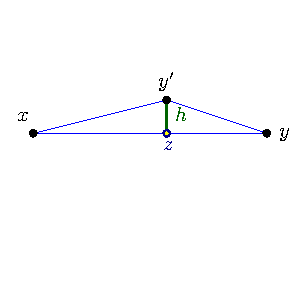
\includegraphics{figs/triangle}%
        \hfill%
        \phantom{}%
        \caption{An illustration of the relative positions of $\px$, $\py$, $\py'$, and $\pz$. The angle of the separating double-wedge guarantees that $\angle \py' \px \py$ is small.}
        \figlab{triangle}
    \end{figure}

    Consider the triangle $\triangle \px \py' \py$, and observe that
    by the double-wedge property
    $\alpha = \angle \py' \px \py \leq \epsA$.  Let $\pz$ be the
    projection of $\py'$ to $\px \py$, and let
    \begin{equation*}
        h%
        =%
        \dY{\py'}{ \pz}%
        =%
        \dY{\px}{\py'} \sin \alpha
        \leq
        \dY{\px}{\py'} \sin \epsA
        \leq%
        \dY{\px}{\py'}  \epsA
        \leq%
        \epsA (1+2 \epsA)\ell
        \leq 
        2 \epsA \ell,
    \end{equation*}
    as $\epsA \in (0,1/10)$, the monotonicity of $\sin$ in this range,
    and as $\sin \epsA \leq \epsA$.
    
    We have that
    $\dY{\px}{\pz} \leq \dY{\px}{\py'} \leq
    (1+2\epsA)\ell$. Similarly, we have
    \begin{equation*}
        \dY{\px}{\pz}%
        =%
        \dY{\px}{\py'} \cos \alpha
        \geq%
        (1-\alpha^2/2)\dY{\px}{\py'} 
        \geq 
        (1-\epsA^2/2)(1-2\epsA)\ell
        \geq
        (1-3\epsA)\ell.
    \end{equation*}


    By the triangle inequality, we have that
    \begin{equation*}
        \dY{\py'}{\py}
        \geq%
        \dY{\px}{\py}
        -\dY{\py'}{\px}        
        \geq%
        \dY{\px}{\py}
        - (1+2\epsA)\ell.
    \end{equation*}
    As for an upper bound, we have
    \begin{align*}
      \dY{\py'}{\py}
      &\leq%
        \dY{\pz}{\py} + h%
        \leq%
        \dY{\px}{\py} - \dY{\px}{\pz} +
        2 \epsA \ell
        \leq
        \dY{\px}{\py} - (1-3\epsA)\ell 
        +2 \epsA \ell
      \\&
      = 
      \dY{\px}{\py} - (1-5\epsA)\ell 
      <%
      \dY{\px}{\py}.
    \end{align*}
    As such, by induction
    $\dGZ{\G}{\py'}{\py} \leq (1+\eps) \dY{\py'}{\py}$.

    We thus have that
    \begin{align*}
      \dGZ{\G}{\px}{\py}%
      &\leq%
        \dGZ{\G}{\px}{\px'} + \dY{\px'}{\py'}
        +
        \dGZ{\G}{\py'}{\py}%
        \leq%
        4\epsA \ell
        +
        \ell
        +
        (1+\eps) \dY{\py'}{\py}
      \\&
      \leq%
      (1+4\epsA) \ell
      +
      (1+\eps) \pth{\bigl.
      \dY{\px}{\py} - (1-5\epsA)\ell }
      \\&
      =%
      \bigl[1+4\epsA
      - (1+\eps)(1-5\epsA)\bigr]\ell 
      +
      (1+\eps)
      \dY{\px}{\py}%
      \\&
      \leq%
      (1+\eps)
      \dY{\px}{\py},
    \end{align*}
    for $\epsA \leq \eps/20$, as
    \begin{math}
        1+4\epsA - (1+\eps)(1-5\epsA)%
        \leq%
        1+\eps/5 - (1+\eps)(1-\eps/4)%
        =%
        \eps/5 -(3/4)\eps + \eps^2/4 < 0,
    \end{math}
    as $\eps < 1$.
\end{proof}

\begin{theorem}
    \thmlab{l:s:squares}%
    %
    Let $\PS$ be a set of $n$ points in the plane, and let
    $\eps \in (0,1)$ be an approximation parameter. The above
    algorithm computes a local $(1+\eps)$-spanner $\G$ for axis
    parallel squares.  The construction time is
    $\Of\pth{\eps^{-3} n \log^2 n}$, and the spanner $\G$ has
    $\Of\pth{\eps^{-3} n \log n}$ edges.
\end{theorem}


%%%%%%%%%%%%%%%%%%%%%%%%%%%%%%%%%%%%%%%%%%%%%%%%%%%%%%%%%%%%%%%%%%%%%%%%%
%%%%%%%%%%%%%%%%%%%%%%%%%%%%%%%%%%%%%%%%%%%%%%%%%%%%%%%%%%%%%%%%%%%%%%%%%
%%%%%%%%%%%%%%%%%%%%%%%%%%%%%%%%%%%%%%%%%%%%%%%%%%%%%%%%%%%%%%%%%%%%%%%%%


\section{Local spanners for fat triangles}

\seclab{triangles}


While local spanners for homothets of an arbitrary convex shape are costly,
if we are given a triangle $\triangle$ with the single constraint that $\triangle$
isn't too ``thin'', one can construct a $\triangle$-local spanner with a number of
edges that does not depend on the spread of the points. See \figref{tri_low_bd} for an illustration of a construction showing that dependency if "thin" triangles are allowed.

\begin{figure}[h]
	\centering
	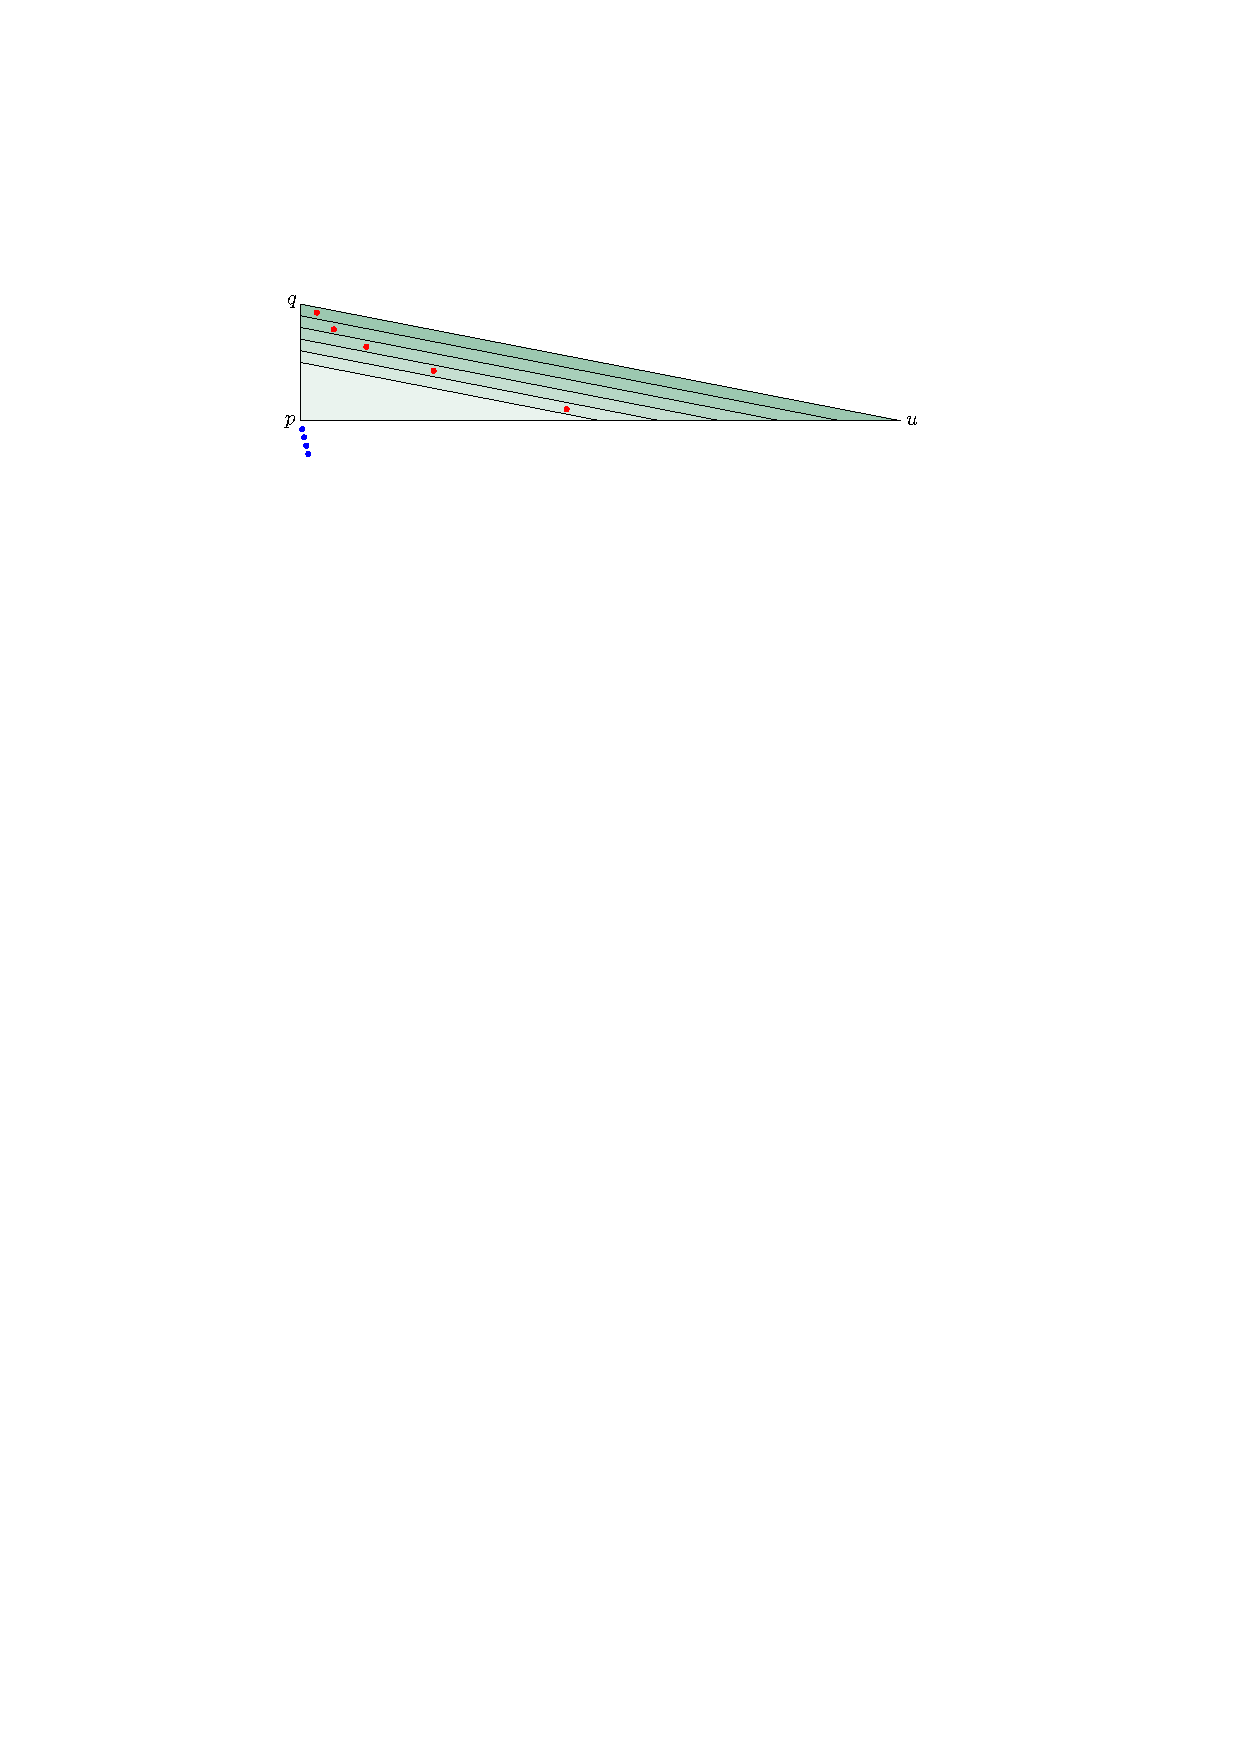
\includegraphics{figs/triangle_lower_bound}
	\caption{For any fixed $t>1$ we can take a "thin" right angle triangle $\triangle$, and create a point set as shown in the figure, such that every blue point must be connected by an edge to many of the red points (which are of exponentially increasing $x$-coordinate) in order to create a $\triangle$-local $t$-spanner.}
	\figlab{tri_low_bd}
\end{figure}


\begin{defn}
	We say that a triangle $\triangle$ is $\alpha$-fat if the smallest angle in $\triangle$ is of size at least $\alpha$.
\end{defn}

\begin{claim}
	For any fixed $\eps \in (0,1)$, there exists a set $\PS$ of $n+\log\Phi$ points with spread $O(\Phi)>> n$ and a triangle $\triangle$, such that the $\triangle$-local $(1+\eps)$-spanner of $\PS$ requires $O\left(n\log\Phi\right)$ edges. 
\end{claim}

\begin{proof}
	First, we describe two sets of points $A$ and $B$ of sizes $n$ and $\log\Phi$ respectively, such that every point in $A$ must be connected to $O(\log\Phi)$ points of $B$ in any $\triangle$-local $(1+\eps)$-spanner for a triangle that we will choose accordingly. 
	Let $A = \{a_i:=(-i, i/n) ~|~ 0\leq i \leq n \}$, and let $B = \{b_i:=(n-i, 1+2^i) ~|~ 1\leq i \leq \log\Phi \}$. It is not hard to see that the spread of $A \cup B$ is indeed $O(\Phi)$.
	
	We now take $\triangle$ to be the right angle triangle with vertices $\pa :=(1,0), \pb :=(1,1)$, and $\pc:=(x,0)$, where $x$ is sufficiently large so that for every $i\in \{1,...,n\}$ there exist a segment parallel to $\overline{\pb\pc}$ with one endpoint on $\overline{\pa\pb}$, and the other on $\overline{\pa\pc}$, that separates $b_i$ and $b_{i-1}$. See \figref{tri_low_bd} for some intuition.
	Notice that for every point $a\in A$ and index $i\in \{0,..,\log\phi\}$, there exist a homothet $\triangle'$ of $\triangle$ such that $B\cap \triangle'=\{b_i,...,b_n\}$. 
	
	We now show that $\dY{a}{b_{i+1}} + \dY{b_{i}}{b_{i+1}} \geq (1+\eps) \dY{a}{b_{i}}$ for $O(n)$ indices. First we make a couple of simple observations:
	
	\begin{enumerate}
		\item $1+\eps \leq 2$,
		\item $\dY{a}{b_{i+1}}\geq 2^{i+1}$,
		\item $\dY{b_{i}}{b_{i+1}} \geq 2^i$,
		\item and $ \dY{a}{b_{i}} \leq 2n + 2^i $.
	\end{enumerate}

	So it is enough to show that for $O(n)$ points in $B$ we have that
	
	$$2^{i+1} + 2^{i} \geq 2(2n + 2^i)$$.
	
	Simplifying a bit we get that the above inequality is true when $i \geq \log(4n)$, and we therefore have that for sufficiently many points of $B$ there must be an edge to every point in $A$. 
	

	
	
\end{proof}
\subsubsection{Construction}
\label{tri_construction}
The input is a point set $\PS$ of $n$ points in the plane, an $\alpha$-fat triangle $\triangle$, and an
approximation parameter $\eps \in (0,1)$. We assume that the smallest angle in $\triangle$ is of size $\alpha$. Let $c_1,c_2$ and $c_3$ be the 3 cones with an apex at the origin that coincide each with one of the angles of $\triangle$ when translating its respective vertex to the origin. We also denote the orthogonal direction to the edge opposite of $\alpha_i$ by $v_i$. See \figref{tri_cones} for an illustration. Let $C_1,C_2$, and $C_3$ be partitions of each of these cones into cones of angle at most $O(\eps)\cdot \alpha$.

For each point $\pa\in\PS$ we create the set of cones $C_\pa$, which is the set of cones $C_1\cup C_2\cup C_3$ translated by $\pa$, and for each $c\in C_\pa$ we connect $\pa$ to the point $\pb\in c$ closest to $\pa$ in an ordering by $v_i$ (where $i$ corresponds to the set $C_i$ that contains the un-translated copy of $c$).
  
%
%For each point we build 
%Let $\eps = ???$.  The algorithm computes a modified version of the $\theta$-graph (see \cite{c-aaspmp-87}). Let $\triangle$ be a triangle, and let $h_1,h_2$ and $h_3$ be the three half planes such that $h_1\cap h_2\cap h_3 = \triangle$, and let $c_{ij}$ be the cone created by taking the intersection of th halfplanes $h_i$ and $h_j$, and translating the apex of that intersection to the origin. We now divide each of the three cones into sub cones of angle at most $\eps$. Let $C$ be the resulted set of cones.
%
%The rest of the construction follows that of the $\theta$-graph with the set of cones $C$. For every $\pa\in\PS$ we create $C_p = \{c+\pa ~|~ c\in C\}$, and for every $c\in C_p$ we connect $\pa$ to the point $c$ whose projection on the bisector of $c$ is closest to $\pa$.


\begin{figure}[h]
	\centering
	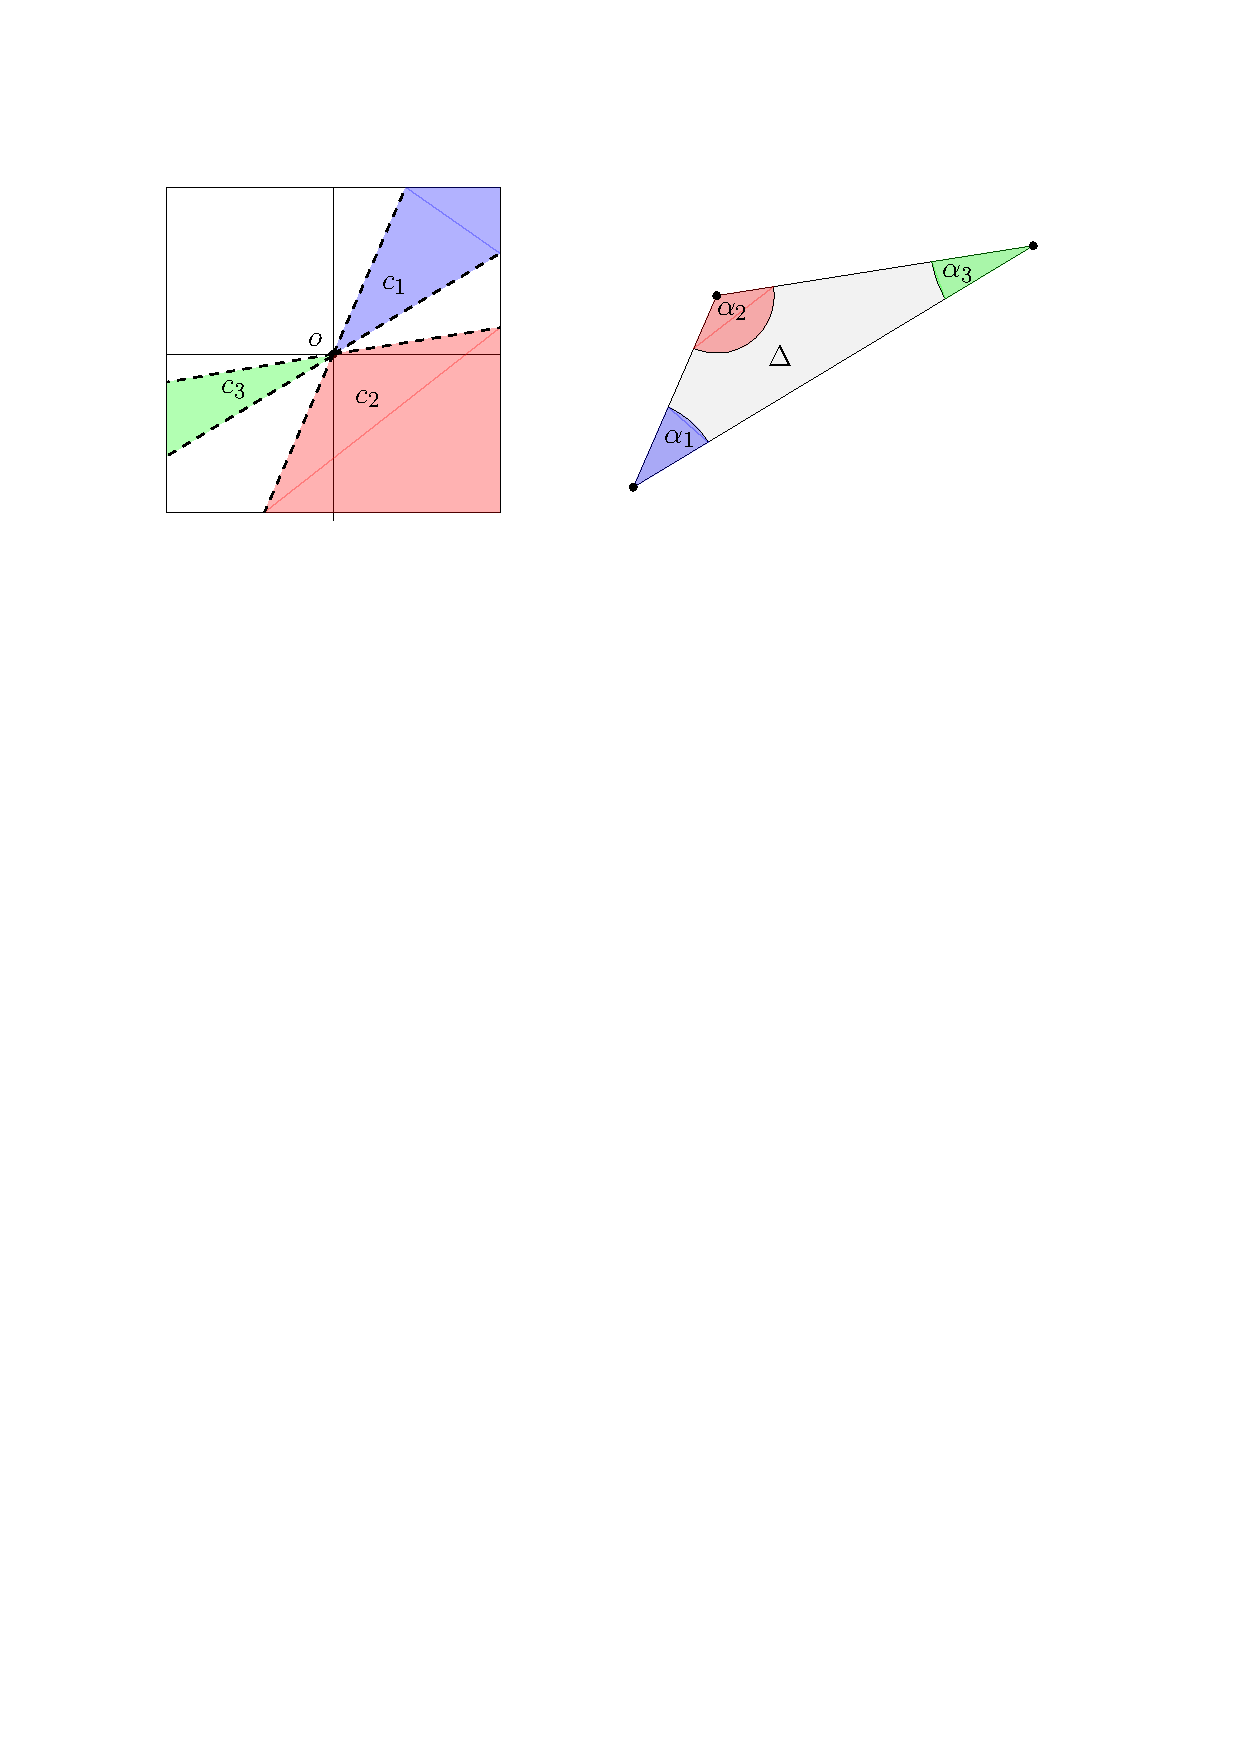
\includegraphics{figs/triangle_cones}
	\caption{For the triangle $\triangle$ with angles $\alpha_1,\alpha_2$, and $\alpha_3$ we create the cones $c_1,c_2$, and $c_3$.}
	\figlab{tri_cones}
\end{figure}
\subsubsection{Analysis}


\paragraph{Shrinking triangles.}
We will need the following lemmas in order to prove the local spanning property of $G$. The first lemma concerns distances between points in the construction above (Subsection \ref{tri_construction}), and the second deals with triangle shrinking.


\begin{lemma}
	\lemlab{cone_edge:triangles}%
	%
	Let $\pa,\pb,\pc\in \PS$ such that the edge $\{\pa, \pc\}$ was added to the graph for the cone $c$ with apex at $\pa$, and such that $\pc\in c$ (as well as $\pa$ and $\pb$).
	
	We get that
	\begin{enumerate}
		\item {
			$
			\dY{\pa}{\pc}%
			+%
			(1+\eps)\dY{\pb}{\pc}%
			\leq%
			(1+\eps)\dY{\pa}{\pb}%
			$
			,and
		}
		\item {
			$
			\dY{\pa}{\pc}%
			\leq%
			\dY{\pa}{\pb}%
			$.
		}
	\end{enumerate}



\end{lemma}

\begin{proof}
	We denote the smallest angle of the triangle $\triangle$ by $\alpha$.
	Consider the triangle $\Delta\pa\pb\pc$ and denote the angles at $\pa,\pb,$ and $\pc$ by $\theta_\pa,\theta_\pb,$ and $\theta_\pc$ respectively.
	
	We now consider two possible cases, either $\dY{\pa}{\pb}\leq \dY{\pa}{\pc}$ or $\dY{\pa}{\pb}> \dY{\pa}{\pc}$. Notice that  since the angle of the cone $c$, and therefore $\theta_\pa$ as well, is smaller   than the smallest angle of $\triangle$, we have that $\dY{\pb}{\pc}\leq    \max \{\dY{\pa}{\pc},\dY{\pa}{\pb}\}$.
	
	$\dY{\pa}{\pb}\leq \dY{\pa}{\pc}$:
	Denote by $\pb'$ the projection of $\pb$ on $\overline{\pa\pc}$. We have that 
	
	$$
	\dY{\pb}{\pb'}%
	=%
	\sin\theta_\pa \dY{\pa}{\pb}%
	=%
	\sin\theta_\pc \dY{\pb}{\pc}%
	\implies%
	\dY{\pb}{\pc}%
	=
	\frac{\sin\theta_\pa}{\sin\theta_\pc}\dY{\pa}{\pb}%
	$$
	
	$$ \dY{\pa}{\pc}%
	=%
	\dY{\pa}{\pb'}%
	+%
	\dY{\pb'}{\pc}%
	=%
	\cos\theta_\pa \dY{\pa}{\pb}%
	+%
	\cos\theta_\pc \dY{\pb}{\pc}%
	=%
	\cos\theta_\pa \dY{\pa}{\pb}%
	+%
	\frac{\sin\theta_\pa}{\sin\theta_\pc}\dY{\pa}{\pb}%
	=%
	(\cos\theta_\pa + \frac{\sin\theta_\pa}{\sin\theta_\pc})\dY{\pa}{\pb}
	$$
	
	We use these equalities and get that:
	
	$$
	\dY{\pa}{\pc}%
	+%
	(1+\eps)\dY{\pb}{\pc}%
	\leq%
	(1+\eps)\dY{\pa}{\pb}%
	$$
	
	$$
	\iff%
	\dY{\pa}{\pb}(\cos\theta_\pa + \frac{\sin\theta_\pa}{\sin\theta_\pc})%
	+%
	(1+\eps)\frac{\sin\theta_\pa}{\sin\theta_\pc}\dY{\pa}{\pb}%
	\leq%
	(1+\eps)\dY{\pa}{\pb}%
	$$
	
	$$
	\iff%
	(\cos\theta_\pa + \frac{\sin\theta_\pa}{\sin\theta_\pc})%
	+%
	(1+\eps)\frac{\sin\theta_\pa}{\sin\theta_\pc}%
	\leq%
	(1+\eps)%
	$$
	
	$$
	\impliedby%
	(1 + \frac{\sin\theta_\pa}{\sin\theta_\pc})%
	+%
	(1+\eps)\frac{\sin\theta_\pa}{\sin\theta_\pc}%
	\leq%
	(1+\eps)%
	$$
	
	$$
	\iff%
	(2+\eps)\frac{\sin\theta_\pa}{\sin\theta_\pc}%
	\leq%
	\eps%
	\iff%
	\frac{\sin\theta_\pa}{\sin\theta_\pc}%
	\leq%
	\frac{\eps}{2+\eps}%
	=%
	O(\eps)%
	$$
	
	The last piece of this part is the fact that point $\pc$ was chosen by being the first point in the cone $c$ encountered by a line parallel to the edge opposite of $\pa$. See the red line and direction in \figref{tri_cone_edge}. This implies that the angle $\theta_\pc$ is at least $\alpha$, and the result then follows.

	$\dY{\pa}{\pb}< \dY{\pa}{\pc}$:
	Denote by $\pc'$ the projection of $\pc$ on $\overline{\pa\pb}$. We have that 
	
	$$
	\dY{\pb}{\pc}%
	\leq%
	\dY{\pc}{\pc'}%
	+%
	\dY{\pb}{\pc'}%
	=%
	\sin\theta_\pa\dY{\pa}{\pc}%
	+%
	(\dY{\pa}{\pb}-\dY{\pb}{\pc'})%
	$$
	
	$$
	\implies%
	\dY{\pb}{\pc}%
	\leq%
	\sin\theta_\pa\dY{\pa}{\pc}%
	+%
	(\dY{\pa}{\pb}-\cos\theta_\pa\dY{\pa}{\pc})%
	$$
	
	$$
	\implies%
	\dY{\pa}{\pc}
	+%
	\frac{1}{\cos\theta_\pa-\sin\theta_\pa}\dY{\pb}{\pc}%
	\leq%
	\frac{1}{\cos\theta_\pa-\sin\theta_\pa}\dY{\pa}{\pb}
	$$
	
	Which means that

	$$
	\dY{\pa}{\pc}%
	+%
	(1+\eps)\dY{\pb}{\pc}%
	\leq%
	(1+\eps)\dY{\pa}{\pb}%
	\iff%
	\frac{1}{\cos\theta_\pa-\sin\theta_\pa}%
	\leq%
	1+\eps%
	$$	
	
	
	Since $\theta_\pa = O(\eps\alpha)$ we get that for a sufficiently large constant the condition $\frac{1}{\cos\theta_\pa-\sin\theta_\pa} \leq 1+\eps$ holds.
	
 	The second part of the lemma is derived from the first:
	
	$$
	\dY{\pa}{\pc}%
	+%
	(1+\eps)\dY{\pb}{\pc}%
	\leq%
	(1+\eps)\dY{\pa}{\pb}%
	\iff%
	\dY{\pb}{\pc}%
	\leq%
	\dY{\pa}{\pb}%
	-%
	\frac{\dY{\pa}{\pc}}{(1+\eps)}%
	\leq%
	\dY{\pa}{\pb}%
	$$
	
	
\end{proof}

\begin{figure}[h]
	\centering
	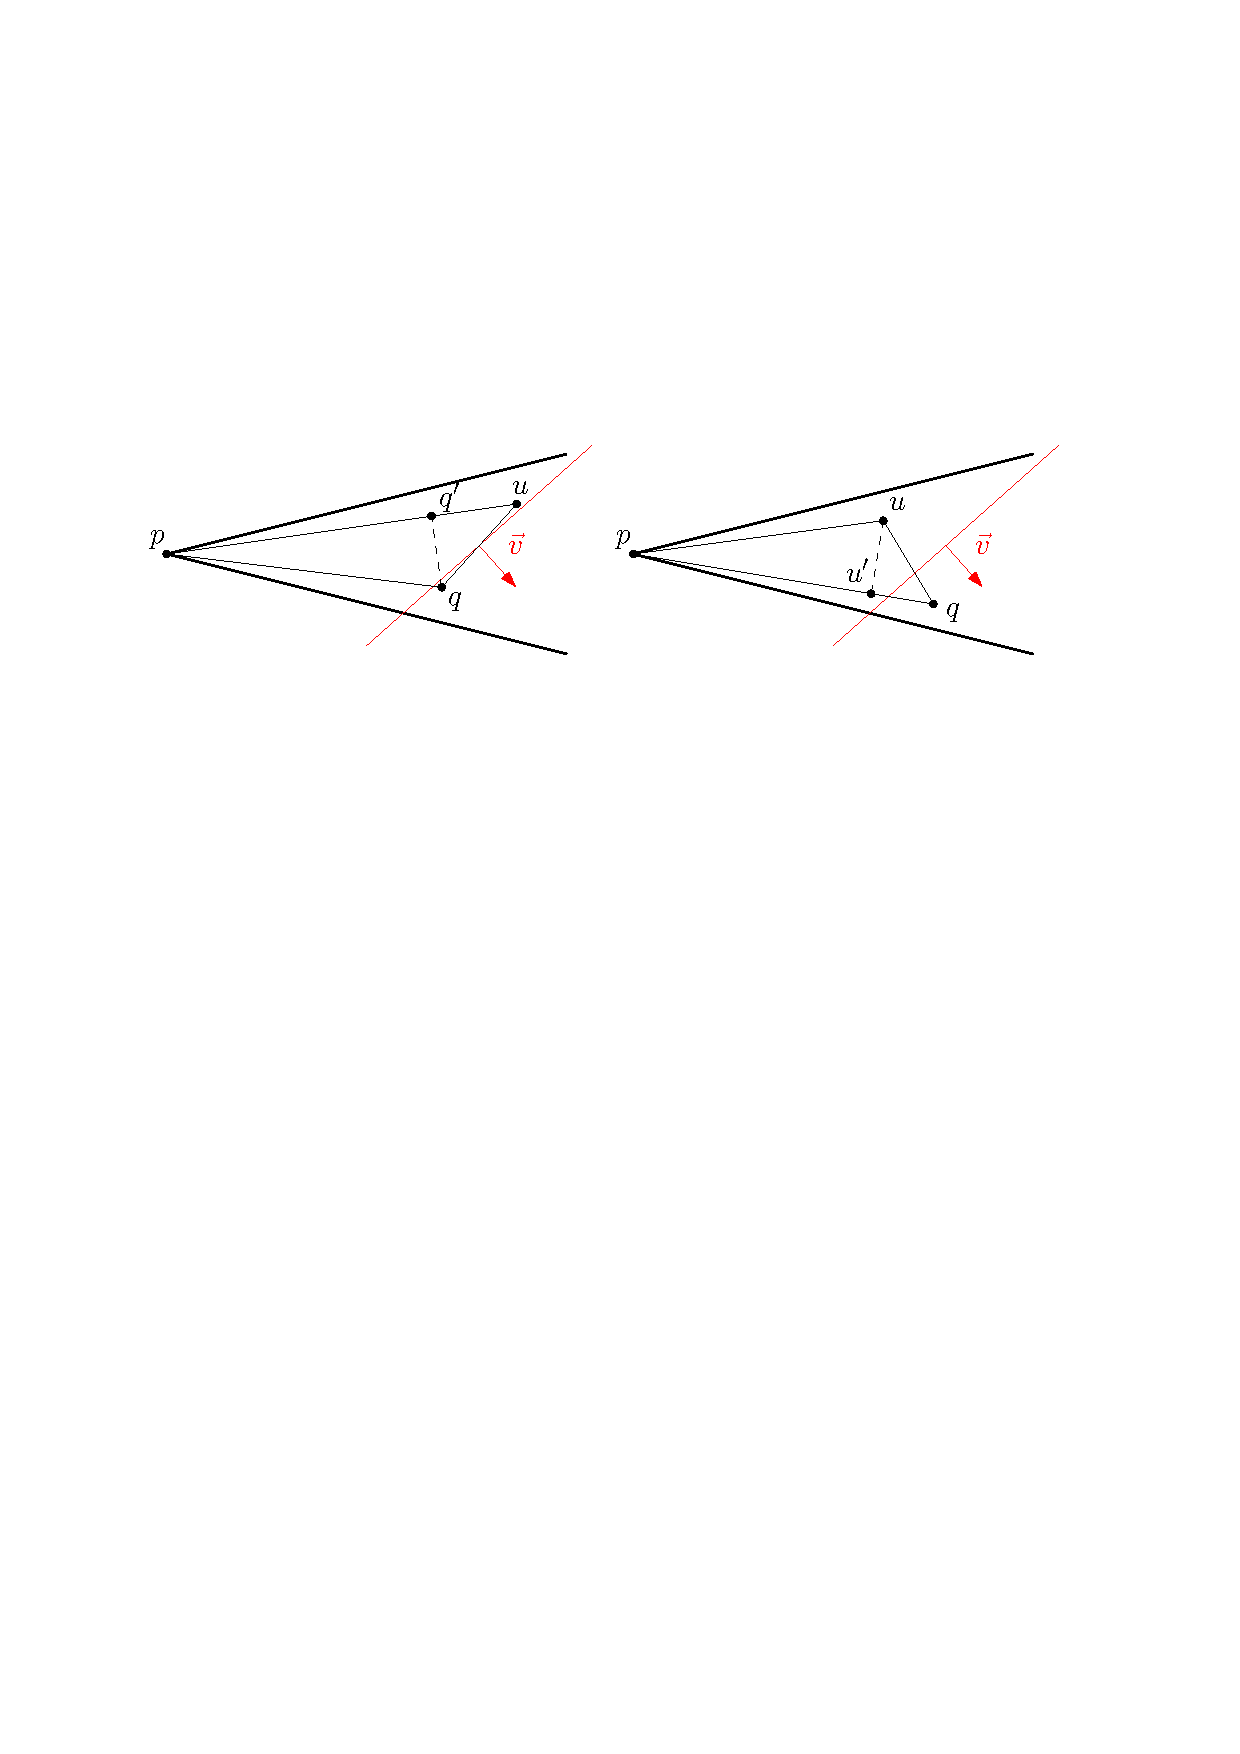
\includegraphics{figs/triangle_cone_edge}
	\caption{The two cases of \lemref{cone_edge:triangles}. The vector used to determine the edge in the cone is shown in red, and marked $\vec{v}$}
	\figlab{tri_cone_edge}
\end{figure}
\subsubsection{Analysis}

We first prove a ``shrinking lemma'' similar to those in \secref{disks} and \secref{squares}.

\begin{lemma}
	\lemlab{shrink:triangles}%
	%
	Let $\triangle$ be a triangle in the plane, and let
	$\pa, \pb$ be two arbitrary points in $\triangle$. Then, there is a
	triangle $\triangle' \subseteq \triangle$ that contains one of $\pa$ and $\pb$ on a vertex, and the other on the edge opposite to that vertex (possibly on a different vertex)
	
\end{lemma}

\begin{proof}
	Choose one of the edges of $\triangle$ and start ``sliding'' it, i.e. incrementally translating it while keeping its slope, shrinking $\triangle$ in the process. We do so until one of $\pa$ or $\pb$ is on the edge. We do the same for the other two edges, choosing the order arbitrarily. The triangle remaining at the end of the process is $\triangle'$, and since we have kept the slopes of all edges we have that $\triangle \sim \triangle'$. We must have that two of the edges were stopped by the same point, which therefore lies on a vertex $v$ of the new triangle. The other point must lie on the edge opposite to $v$, since otherwise one of the edges can still be moved to shrink $\triangle'$. See \figref{shrink_tri}.
	
\end{proof}

\begin{figure}[h]
	\centering
	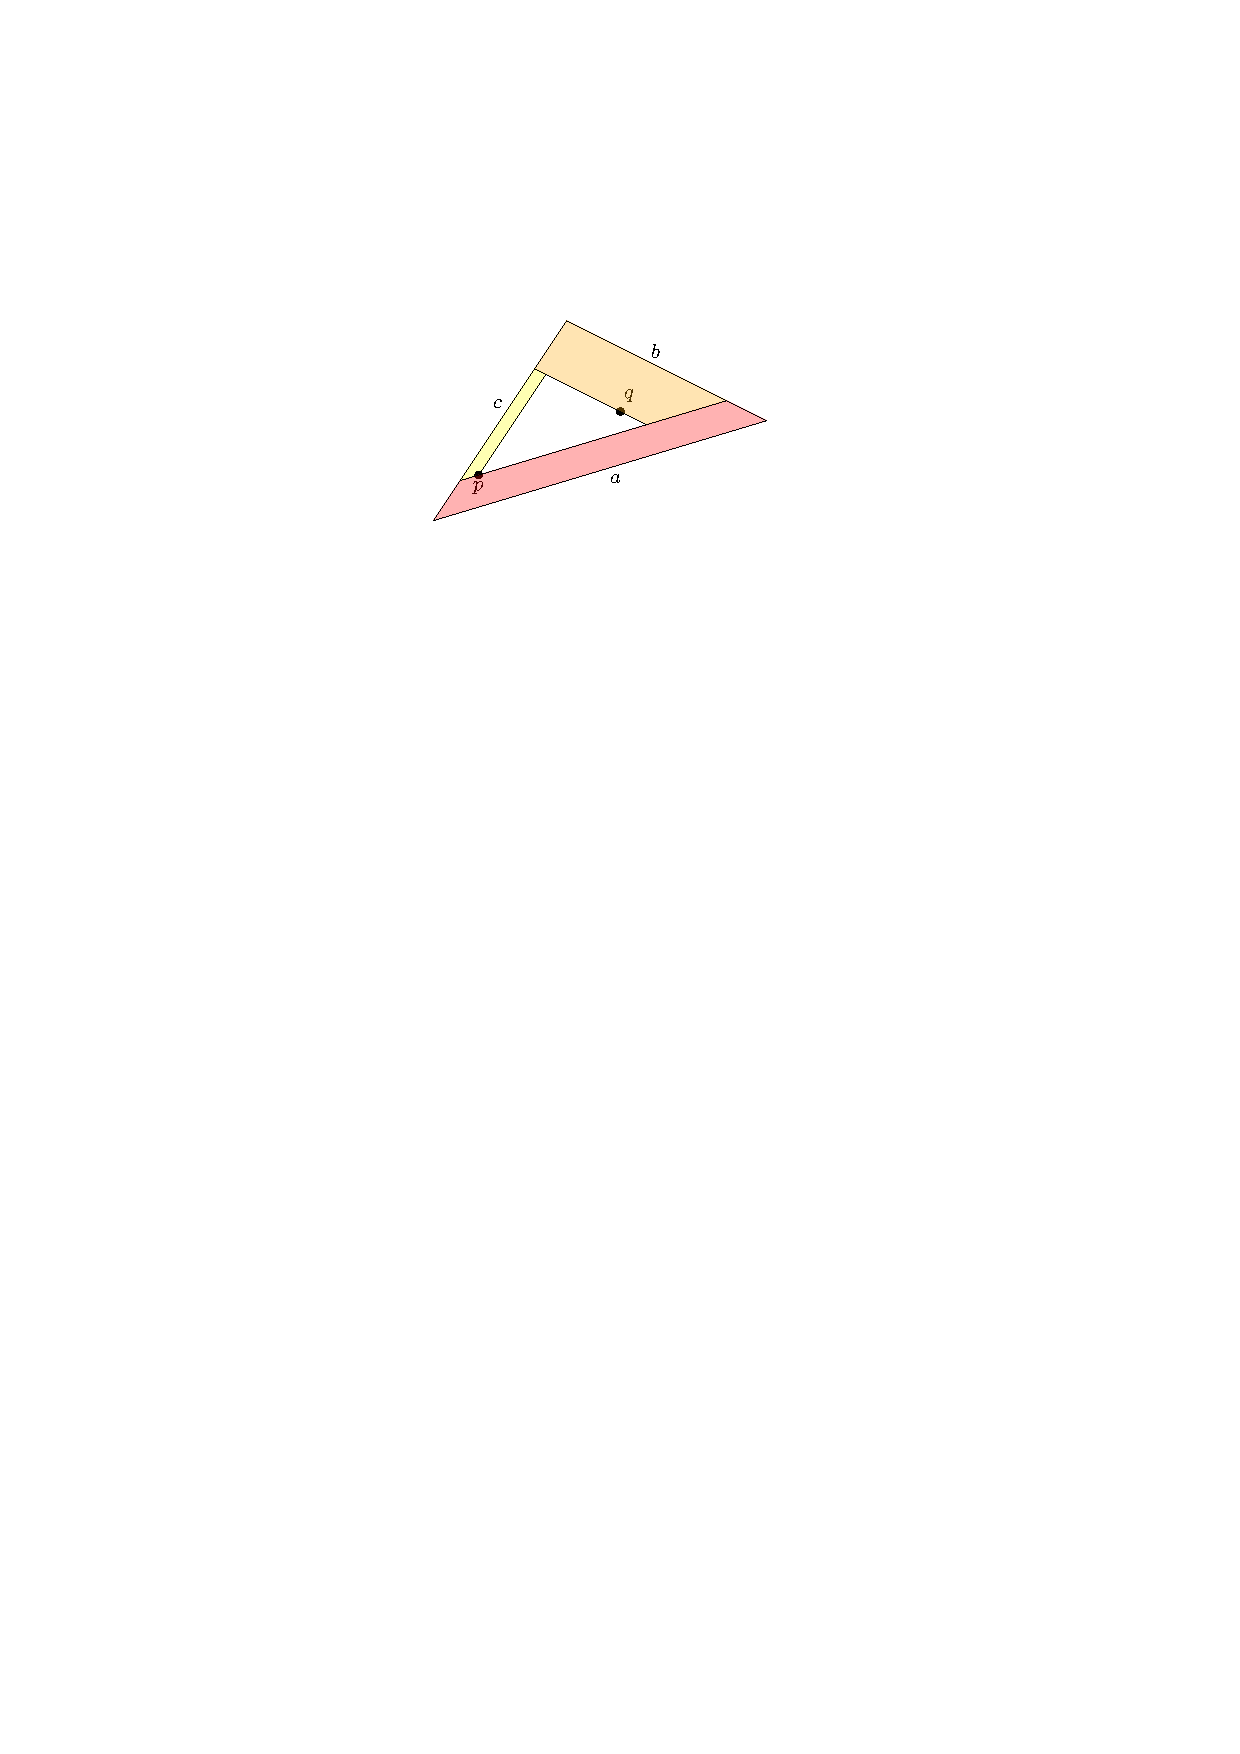
\includegraphics{figs/shrink_tri}
	\caption{The edges are moved in the order $a,b,c$, resulting in the required similar triangle.}
	\figlab{shrink_tri}
\end{figure}



\paragraph{Local spanner property.}
\begin{lemma}
	\lemlab{local_span:triangles}%
	%
	For a triangle $\triangle$, denote the graph constructed by the process above (Subsection \ref{tri_construction}) by $G$. for any homothet of $\triangle$, and any two points $\pa, \pb \in \PS$ in the homothet, we have a $(1+\eps)$-path in
	$\restrictY{\G}{\triangle}$.
\end{lemma}



\begin{proof}
	We slightly abuse notation and denote the homothet by $\triangle$. We prove the existence of the $(1+\eps)$-path by induction over the rank of the distance $\dY{\pa}{\pb}$. The closest pair $\pa',\pb'$ must be connected in $G$, as otherwise we have that $\dY{\pa'}{\pc'}+\dY{\pb'}{\pc'}\geq 2 \dY{\pa'}{\pb'}$ regardless of the angle of the cone, a contradiction to  \lemref{cone_edge:triangles}.
	
	For any other pair $\pa,\pb\in PS\cap \triangle$ we have from \lemref{shrink:triangles} that there exists a homothet $\triangle'\subseteq \triangle$ with one of the two points, say $\pa$, at a vertex, and the other on the opposite edge. We therefore have a cone $c$ with apex at $\pa$ such that $\pb\in c\cap \triangle'$. If $\pa\pb$ is an edge in $G$ then we are done. Otherwise, we have a vertex $\pc\in c$ such that $\pa\pb$ is an edge in $G$, and we therefore get from \lemref{cone_edge:triangles} that $\dY{\pb}{\pc}\leq \dY{\pa}{\pb}$ and therefore, by the induction hypothesis, we have that there exists a $(1+\eps)$ path between $\pc$ and $\pb$ in $G$. From the same lemma it also follows that $\dY{\pa}{\pc}+(1+\eps)\dY{\pb}{\pc}\leq(1+\eps)\dY{\pa}{\pb}$, and thus we get the existence of a $(1+\eps)$ path between $\pa$ and $\pb$ as well.
	
\end{proof}


\paragraph{Size and running time.}
Let $G$ be the graph constructed by the procedure described above.


\begin{theorem}
	\thmlab{l:s:triangle}%
	%
	Let $\PS$ be a set of $n$ points in the plane, and let
	$\eps \in (0,1)$ be an approximation parameter. The above
	algorithm computes a local $(1+\eps)$-spanner $\G$ for homothets of an $\alpha$-fat triangle $\triangle$.
	The construction time is
	$O\left(\frac{1}{\alpha\eps}n\log n\right)$, and the spanner $\G$ has
	$O\left(\frac{1}{\alpha\eps}n\right)$ edges.
\end{theorem}

\begin{proof}
	The local-spanning property is proven in \lemref{local_span:triangles}, and we are only left with bounding the size and the running time of the algorithm. The bound on the size is immediate from the construction, as every point $\pa$ is the apex of $O\left( \frac{2\pi}{\eps\alpha} \right)$ cones, each giving rise to a single edge incident to $\pa$.
	The construction time is bounded by the construction time for a $\theta$-graph with cone size $\alpha\eps$, which is $O\left(\frac{1}{\alpha\eps}n\log n\right)$ (\cite{c-aaspmp-87})
\end{proof}





%%%%%%%%%%%%%%%%%%%%%%%%%%%%%%%%%%%%%%%%%%%%%%%%%%%%%%%%%%%%%%%%%%%%%%%%%
%%%%%%%%%%%%%%%%%%%%%%%%%%%%%%%%%%%%%%%%%%%%%%%%%%%%%%%%%%%%%%%%%%%%%%%%%
%%%%%%%%%%%%%%%%%%%%%%%%%%%%%%%%%%%%%%%%%%%%%%%%%%%%%%%%%%%%%%%%%%%%%%%%%

\section{Weak local spanners for convex regions %
   with bounded aspect ratio}
\seclab{convex regions}

We would like to build local spanners (of subquadratic size) for
axis-parallel rectangles, but as \figref{bad:rectangles} shows, there
is no hope of achieving this. As such, we need to somewhat change the
requirements, and instead describe a weak local spanner for this case.
The exact meaning of the weakness of the spanner, parameterized by
$\delta$ is given below.

\begin{figure}
    \centerline{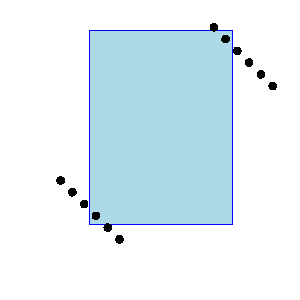
\includegraphics{figs/local_rectangles}}
    \caption{There are quadratic number of pairs of points that has to
       be connected in any local spanner for axis parallel
       rectangles. Indeed, for any point in the top diagonal and
       bottom diagonal, there is an axis parallel rectangle that
       contains only these two points. This holds even if we restrict
       ourselves to fat rectangles of similar size.}
    \figlab{bad:rectangles}
\end{figure}


% \subsection{Shrinking the area of service}

% \subsubsection{Shrinking by the diameter}

\begin{defn}
    Given a convex region $\body$, let
    \begin{equation*}
        \shrinkDY{\body}{\delta}%
        =%
        \Set{ \pa \in \body }{ \dsY{\pa}{ \Re^2 \setminus \body} \geq \delta \cdot
           \diameterX{\body}}.        
    \end{equation*}
    Formally, $\shrinkDY{\body}{\delta}$ is the Minkowski difference
    of $\body$ with a disk of radius $\delta \cdot \diameterX{\body}$.
\end{defn}


\begin{defn}
    Consider a (bounded) set $\body$ in the plane. Let $\rinX{\body}$
    be the radius of the largest disk contained inside $\body$.
    Similarly, $\routX{\body}$ is the smallest radius of a disk
    containing $\body$.

    The \emphi{aspect ratio} of a region $\body$ in the plane is
    $\arX{\body} = \routX{\body}/\rinX{\body}$. Given a family $\FF$
    or regions in the plane, its \emphw{aspect ratio} is
    $\arX{\FF} = \max_{\body \in \FF} \arX{\body}$.
\end{defn}

Note, that if a convex region $\body$ has bounded aspect ratio, then
$\shrinkDY{\body}{\delta}$ is similar to the result of scaling $\body$
by a factor of $1-O(\delta)$. On the other hand, if $\body$ is long
and skinny, say is has width smaller than
$2 \delta \cdot \diameterX{\body}$, then $\shrinkDY{\body}{\delta}$ is
empty.


\begin{lemma}
    \lemlab{w:l:s:regions}%
    %
    Given a set $\PS$ of $n$ points in the plane, and parameters
    $\delta, \eps \in (0,1)$.  One can construct a graph $\G$ over
    $\PS$, in $\Of( (\eps^{-1} + \delta^{-2}) n \log n)$ time, and
    with $\Of\bigl( (\eps^{-1} + \delta^{-2}) n \bigr) $ edges, such
    that for any (bounded) convex $\body$ in the plane, we have that
    for any two points
    $\pa, \pb \in \PS \cap \shrinkDY{\body}{\delta}$ the graph
    $\restrictY{ \body }{\PS}$ has $(1+\eps)$-path between $\pa$ and
    $\pb$.
\end{lemma}

\begin{proof}
    Let $\epsA = \min( \eps, \delta^2)$. Construct, in
    $\Of(\epsA^{-1} n \log n)$ time, a standard $(1+\epsA)$-spanner $\G$
    for $\PS$ using $\Of( \epsA^{-1} n)$ edges \cite{ams-dagss-99}.

    So, consider any body $\body \in \FF$, and any two vertices
    $\pa, \pb \in \PS \cap \body'$, where
    $\body'=\shrinkDY{\body}{\delta}$. Let $\ell = \dY{\pa}{\pb}$, 
    let $\pi$ be the shortest path between $\pa$ and $\pb$ in $\G$, and let
    $\Elp$ be the locus of all points $\pc$, such that
    $\dY{\pa}{\pc} + \dY{\pc}{\pb} \leq (1+\epsA) \ell$. The region
    $\Elp$ is an ellipse that contains $\pi$. The furthest point from
    the segment $\pa\pb$ in this ellipse is realized by the co-vertex
    of the ellipse. Formally, it is one of the two intersection points
    of the boundary of the ellipse with the line orthogonal to
    $\overline{\pa \pb}$ that passes through the middle point $\cen$ of this
    segment, see \figref{ellipse}. Let $\pz$ be one of these points.

    \begin{figure}[h]
        \centerline{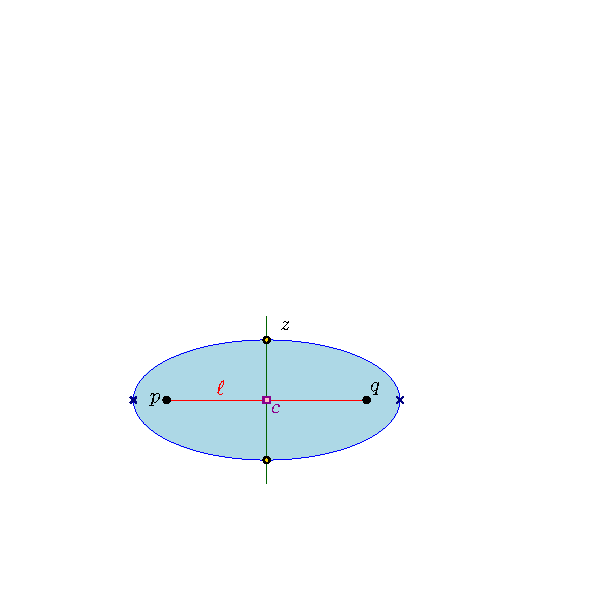
\includegraphics{figs/ellipse}}
        \caption{}
        \figlab{ellipse}
    \end{figure}

    We have that
    \begin{math}
        \dY{\pa}{\pz} = (1+\epsA)\ell/2.
    \end{math}
    Setting $h = \dY{\pz}{\cen}$, we have that
    \begin{equation*}
        h%
        =%
        \sqrt{\dY{\pa}{\pz}^2 - \dY{\pa}{\cen}^2 }
        =%
        \frac{\ell}{2} \sqrt{(1+\epsA)^2 - 1}
        =%
        \frac{\sqrt{\epsA (2+\epsA)}}{2} \ell%
        \leq 
        \sqrt{\epsA} \ell
        \leq 
        \sqrt{\epsA}\cdot \diameterX{\body}.
    \end{equation*}
    as $\ell \leq \diameterX{\body'} \leq \diameterX{\body}$.

    For any point $\px \in \body'$, we have that
    $\dsY{\px}{\Re^2 \setminus \body} \geq \delta \cdot \diamX{\body}$.  As
    such, to ensure that $\pi \subseteq \Elp \subseteq \body$, we need
    that
    \begin{math}
        \delta \cdot \diamX{\body} \geq h,
    \end{math}
    which holds if
    \begin{math}
        \delta \cdot \diamX{\body} \geq \sqrt{\epsA} \cdot  \diameterX{\body}.
    \end{math}
    This in turn holds if $\epsA \leq \delta^2$. Namely, we have the
    desired properties if $\epsA = \min( \eps, \delta^2)$.
\end{proof}


% Before dwelling into the construction, we start with presenting a
% new pair decomposition that would be useful for our (nefarious)
% purposes, and is of independent interest.

%%%%%%%%%%%%%%%%%%%%%%%%%%%%%%%%%%%%%%%%%%%%%%%%%%%%%%%%%%%%%%%%%%%%%%%%%
%%%%%%%%%%%%%%%%%%%%%%%%%%%%%%%%%%%%%%%%%%%%%%%%%%%%%%%%%%%%%%%%%%%%%%%%%
%%%%%%%%%%%%%%%%%%%%%%%%%%%%%%%%%%%%%%%%%%%%%%%%%%%%%%%%%%%%%%%%%%%%%%%%%

\section{Weak local spanners for axis-parallel rectangles}
\seclab{rectangles}
\subsection{Quadrant separated pair decomposition}

For points $\pa = (p_1, \ldots, p_d)$ and $\pb = (q_1, \ldots, q_d)$
in $\Re^d$, let $\pa \prec \pb$ denotes that $\pb$ \emphi{dominates}
$\pa$ coordinate-wise. That is $p_i < q_i$, for all $i$. More
generally, let $\pa <_i \pb$ denote that $\pa_i < \pb_i$. For two
point sets $\PSX, \PSY \subseteq \Re^d$, we use $\PSX <_i \PSY$ to
denote that $\forall \px \in \PSX, \py \in \PSY \quad \px <_i \py$.
In particular $\PSX$ and $\PSY$ are \emphw{$i$-coordinate separated}
if $\PSX <_i \PSY$ or $\PSY <_i \PSX$. A pair $\{ \PSX, \PSY\}$ is
\emphi{quadrant-separated}, if $\PSX$ and $\PSY$ are $i$-coordinate
separated, for $i=1,\ldots, d$.

A \emphi{quadrant-separated pair decomposition} of a point set
$\PS \subseteq \Re^d$, is a pair decomposition (see
\defref{pair:decomposition})
$\WS = \bigl\{ \{ \PSX_1, \PSY_1 \}, \ldots, \{ \PSX_s, \PSY_s \}
\bigr\}$ of $\PS$, such that $\{ \PSX_i, \PSY_i\}$ are
quadrant-separated for all $i$.


\begin{lemma}
    \lemlab{d:1}%
    %
    Given a set $\PS$ of $n$ points in $\Re$, one can compute, in
    $\Of( n \log n)$ time, a \QSPD of $\PS$ with $\Of(n)$ pairs, and of
    total weight $\Of( n \log n)$.
\end{lemma}
\begin{proof}
    If $\PS$ is a singleton then there is nothing to do. If
    $\PS = \{ \pa, \pb \}$, then the decomposition is the pair formed
    by the two singleton points.

    Otherwise, let $x$ be the median of $\PS$, such that
    $\PS_{\leq x} = \Set{ \pa \in \PS }{\pa \leq x}$ contains exactly
    $\ceil{n/2}$ points, and $\PS_{> x} = \PS \setminus \PS_{\leq x}$
    contains $\floor{n/2}$ points. Construct the pair
    $\Pair = \{ \PS_{\leq x}, \PS_{> x} \}$, and compute recursively a
    \QSPD{}s $\QS_{\leq x}$ and $\QS_{> x}$ for $\PS_{\leq x}$ and
    $\PS_{> x}$, respectively. The desired \QSPD is
    \begin{math}
        \QS_{\leq x} \cup \QS_{> x} \cup \{ \Pair \}.
    \end{math}
    The bounds on the size and weight of the desired \QSPD are
    immediate.
\end{proof}


\begin{lemma}
    Given a set $\PS$ of $n$ points in $\Re^d$, one can compute, in
    $\Of( n \log^d n)$ time, a \QSPD of $\PS$ with $\Of(n \log^{d-1} n)$
    pairs, and of total weight $\Of( n \log^d n)$.
\end{lemma}
\begin{proof}
    The construction algorithm is recursive on the dimensions, using
    the algorithm of \lemref{d:1} in one dimension.

    The algorithm computes a value $\alpha_d$ that partitions the values of the points' $d$\th coordinates roughly equally (and is
    distinct from all of them), and let $h$ be a hyperplane parallel
    to the first $d-1$ coordinate axes, and having value $\alpha_d$ in
    the $d$\th coordinate.

    Let $\PS_{\uparrow}$ and $\PS_{\downarrow}$ be the subset of
    points of $\PS$ that are above and below $h$, respectively. The
    algorithm recursively computes \QSPD{}s $\QS_\uparrow$ and
    $\QSdown$ for $\PSup$ and $\PS_{\downarrow}$, respectively.  Next,
    the algorithm projects the points of $\PS$ on $h$, let $\PS'$
    be the resulting $d-1$ dimensional point set (after we ignore the
    $d$\th coordinate), and recursively computes a \QSPD $\QS'$ for $\PS'$.

    
    For a point set $\PSX' \subseteq \PS'$, let $\liftX{\PSX'}$ be the
    subset of points of $\PS$ whose projection on $h$ is $\PSX'$.
    The algorithm now computes the set of pairs
    \begin{equation*}
        \widehat{\QS}%
        =%
        \Set{\Bigl.
           \{ \liftX{ \PSX'} \cap \PSup , \liftX{ \PSY' } \cap \PSdown
           \}, \,\,
           \{ \liftX{ \PSX'} \cap \PSdown , \liftX{ \PSY' } \cap \PSup
           \}
        }%
        { \{ \PSX', \PSY' \} \in \QS'}     .
    \end{equation*}
    The desired \QSPD is $\widehat{\QS} \cup \QSup \cup \QSdown$.

    To observe that this is indeed a \QSPD, observe that all the pairs
    in $\QSup, \QSdown$ are quadrant separated by induction. As for
    pairs in $\widehat{\QS}$, they are quadrant separated in the first
    $d-1$ coordinates by induction on the dimension, and separated in
    the $d$ coordinate since one side of the pair comes from $\PSup$,
    and the other side from $\PSdown$.

    As for coverage, consider any pair of points $\pa, \pb \in \PS$,
    and observe that the claim holds by induction if they are both in
    $\PSup$ or $\PSdown$. As such, assume that $\pa \in \PSup$ and
    $\pb \ni \PSdown$. But then there is a pair
    $\{\PSX', \PSY'\} \in \QS'$ that separates the two projected
    points in $h$, and clearly one of the two lifted pairs that
    corresponds to this pair quadrant-separates $\pa$ and $\pb$ as
    desired.

    The number pairs in the decomposition is
    \begin{math}
        N(n,d) = 2N(n,d-1) + 2N\pth{ n/2, d }
    \end{math}
    with $N(n,1) = O(n)$. The solution to this recurrence is
    $N(n,d) = O( n \log^{d-1} n)$.  The total weight of the
    decomposition is
    \begin{math}
        W(n,d) = 2W(n,d-1) + 2W\pth{ n/2, d }
    \end{math}
    with $W(n,1) = O(n \log n)$. The solution to this recurrence is
    $W(n,d) = O( n \log^{d} n)$. Clearly, this also bounds the
    construction time.
\end{proof}

%%%%%%%%%%%%%%%%%%%%%%%%%%%%%%%%%%%%%%%%%%%%%%%%%%%%%%%%%%%%%%%%%%%%%%

\subsection{Weak local spanner for axis parallel rectangles}

For a parameter $\delta \in (0,1)$, and an interval $I = [b,c]$, let
$(1-\delta)I = [t - (1-\delta)r, t+ (1-\delta)r]$ be the shrinking of
$I$ by a factor of $1-\delta$, where $t = (b+c)/2$, and $r = (c-b)/2$.


Let $\Rects$ be the set of all axis parallel rectangles in the
plane. For a rectangle $\rect \in \Rects$, with $\rect = I \times J$,
let $(1-\delta)\rect = (1-\delta)I \times (1-\delta)J$ denote the
rectangle resulting from shrinking $\rect$ by a factor of $1-\delta$.

\begin{defn}
    Given a set $\PS$ of $n$ points in the plane, and parameters
    $\eps, \delta \in (0,1)$, a graph $\G$ is a
    \emphw{$(1-\delta)$-local $(1+\eps)$-spanner} for rectangles, if
    for any axis-parallel rectangle $\rect$, we have that
    $\restrictY{\G}{\rect}$ is a $(1+\eps)$-spanner for all the points
    in $(1-\delta)\rect \cap \PS$.
\end{defn}

Observe that rectangles in $\Rects$ might be quite ``skinny'', so the
previous notion of shrinkage used before are not useful in this case.

\subsubsection{Construction for a single quadrant separated pair}
\seclab{pair:edges}

\begin{figure}[t]
    \centering%
    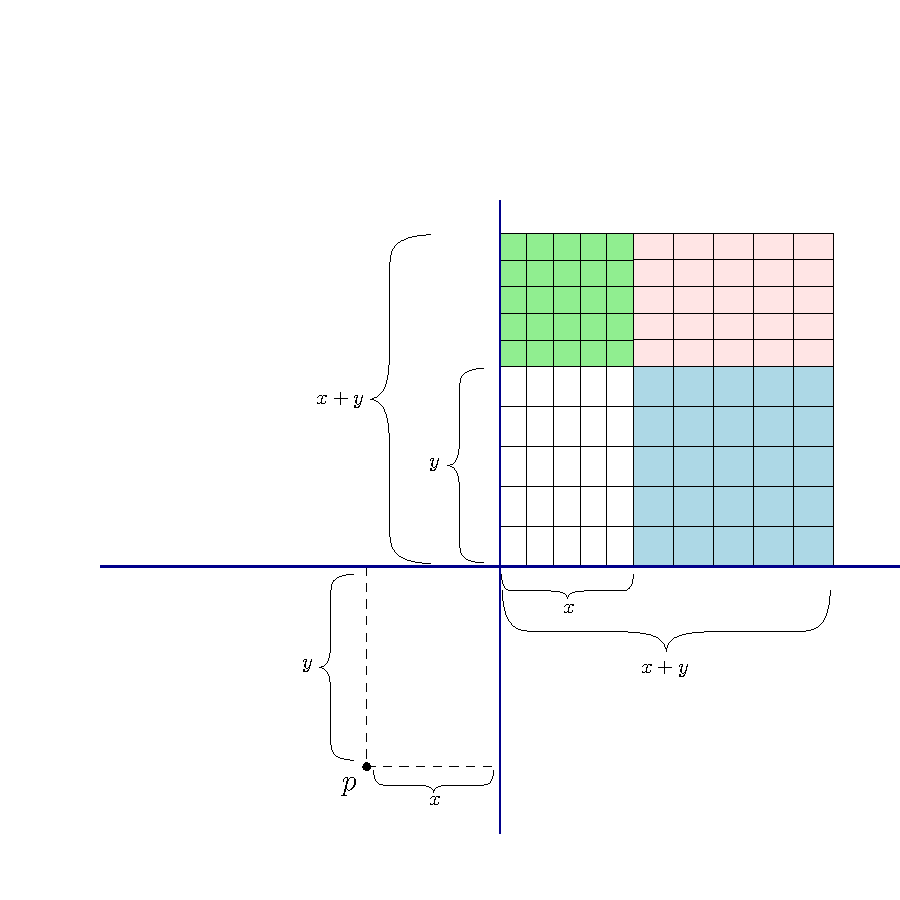
\includegraphics{figs/grid_construction}%
    \caption{The construction of the grid $\grid(\pa,\Pair)$ for a
       point $\pa=(-x,-y)$ and a pair $\Pair$.
       %We are not showing the
       %subrectangles of $\rectA_\nearrow$ as they are not being used
       %in the construction. 
   }
    \figlab{grid}%
\end{figure}

Consider a pair $\Pair = \{\PSX, \PSY \}$ in a \QSPD of $\PS$. The set
$\PSX$ is quadrant-separated from $\PSY$. That is, there is a point
$\cen_\Pair$, such that $\PSX$ and $\PSY$ are contained in two
opposing quadrants in the partition of the plane formed by the
vertical and horizontal line through $\cen_\Pair$.

For simplicity of exposition, assume that $\cen_\Pair = (0,0)$, and
$\PSX \prec (0,0 ) \prec \PSY$. That is, the points of $\PSX$ are in
the negative quadrant, and the points of $\PSY$ are in the positive
quadrant.

Consider a point $\pa = (-x,-y) \in \PSX$. Its \emphw{set of clients} in $\PSY$,
is
\begin{equation*}
    \clientsY{\pa}{\PSY}%
    =%
    \Set{ \pb \in \PSY }{ \dZ{1}{\pb}{\cen_\Pair}  \leq
       \dZ{1}{\pa}{\cen_\Pair}}.
\end{equation*}

We construct a non-uniform grid $\grid(\pa, \Pair)$ in the square
$[0,x+y]^2$.  To this end, we first partition it into four
subrectangles
\begin{equation*}
    \begin{array}{l|l}
      \rectA_\nwarrow = [0,x] \times [y,x+y]
      &
        \rectA_\nearrow = [x,x+y] \times [y,x+y]\Bigr.\\
      \hline
      \rectA_{\swarrow} = [0,x]\times [0,y]
      &
        \rectA_\searrow = [x,x+y] \times [0,y].\Bigr.\\
    \end{array}
\end{equation*}


Let $\gConst \geq 4/\eps + 4/\delta$ be an integer number.  We partition each of these rectangles into a
$\gConst \times \gConst$ grid, where each cell is a copy of the rectangle scaled by a factor of $1/\gConst$.  See \figref{grid}. This grid has $\Of(\gConst^2)$
cells. For a cell $\cell$ in this grid, let $\PSY \cap \cell$ be the
points of $\PSY$ contained in it. We connect $\pa$ to the left-most
and bottom-most points in $\PSY \cap \cell$. This process generates
two edges in the constructed graph for each grid cell, and
$\Of( \gConst^2)$ edges overall.

The algorithm repeats this construction for all the points
$\pa \in \PSX$, and does the symmetric construction for all the points
of $\PSY$.


\subsubsection{The construction algorithm}

The algorithm computes a \QSPD $\WS$ of $\PS$. For each pair
$\Pair \in \WS$, the algorithm generates edges for $\Pair$ using the
algorithm of \secref{pair:edges} and adds them to the generated
spanner $\G$.




\begin{figure}
    \phantom{}\hfill%
    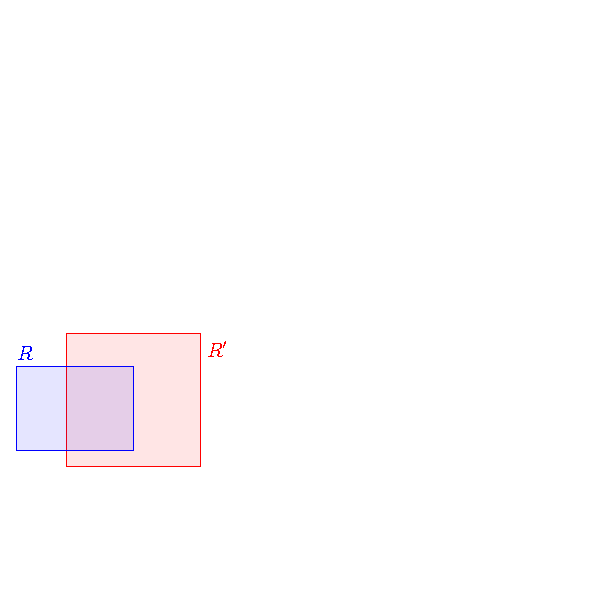
\includegraphics[page=1]{figs/expand}%
    \hfill%
    \includegraphics[page=2]{figs/expand}%
    \hfill\phantom{}%
    \caption{}
    \figlab{x:expand}
\end{figure}


\subsubsection{Correctness}

% For a set $Z \subseteq \Re^2$, let
% $Z_y = \Set{ y \in \Re}{ \exists (x,y) \in Z}$ be the projection of
% $Z$ to the $y$ axis. The set $Z_x$ is defined symmetrically. For
% rectangles $\rect, \rect'$, the set

For a rectangle $\rect$, let
$\xSlabX{\rect} = \Set{(x,y)\in \Re^2}{\exists (x',y) \in \rect}$ be
its expansion into a horizontal slab. Restricted to a rectangle
$\rect'$, the resulting set is $\xSlabX{\rect} \cap \rect'$, depicted
in \figref{x:expand}.  Similarly, we denote
$\ySlabX{\rect} = \Set{(x,y)\in \Re^2}{\exists (x,y') \in \rect}$.

\begin{figure}[h]
    \includegraphics[page=2]{figs/grid_2}%
    \hfill%
    \includegraphics[page=3]{figs/grid_2}%
    \hfill%
    \includegraphics[page=4]{figs/grid_2}
    \caption{}
    \figlab{grid:2}
\end{figure}
\begin{lemma}
    \lemlab{cases}%
    %
    Assume that $\gConst \geq \ceil{20/\eps + 20/\delta}$.  Consider a
    pair $\Pair = \{\PSX, \PSY \}$ in the above construction, and a
    point $\pa =(-x,-y) \in \PSX$, and its associated grid
    $\grid = \grid(\pa, \Pair)$. Consider any axis
    parallel rectangle $\rect$, such that
    $\pa \in (1-\delta)\rect = I\times J$, and $(1-\delta)\rect$
    intersects a cell $\cell \in \grid$. We have that:
    \begin{compactenumI}
        \smallskip%
        \item \itemlab{i:c} If $\cell \subseteq (1-\delta)\rect$ then
        $(1-\delta)^{-1} \cell \subseteq \rect$.

        \item \itemlab{small:diam}
        $\diameterX{\cell} \leq (\eps/4) \dsY{\pa}{\cell}$.

        % \smallskip%
        \item \itemlab{x:bigger} If $x \geq y$ and
        $\cell \subseteq \rect_\swarrow \cup \rect_\searrow$ then
        $(1-\delta)^{-1} \cell \subseteq \rect$.

        \item \itemlab{y:bigger} If $x \leq y$ and
        $\cell \subseteq \rect_\swarrow \cup \rect_\nwarrow$ then
        $(1-\delta)^{-1} \cell \subseteq \rect$.

        \smallskip%
        \item \itemlab{n:w} If $x \geq y$ and
        $\cell \subseteq \rect_\nwarrow$, then
        $(1-\delta)^{-1} \bigl(\xSlabX{ (1-\delta)\rect} \cap \cell
        \bigr) \subseteq \rect$.

        \smallskip%
        \item \itemlab{s:e} If $x \leq y$ and
        $\cell \subseteq \rect_\searrow$, then
        $(1-\delta)^{-1} \Bigl(\ySlabX{\bigl( (1-\delta)\rect \bigr)}
        \cap \cell \Bigr) \subseteq \rect$.
    \end{compactenumI}
\end{lemma}
\begin{proof}
    \itemref{i:c} is immediate, \itemref{y:bigger} and \itemref{s:e}
    follows by symmetry from \itemref{x:bigger} and \itemref{n:w},
    respectively.

    \smallskip%
    \noindent%
    \itemref{small:diam} We have that
    \begin{math}
        \diameterX{\cell}%
        \leq%
        (x+y) /\gConst%
        \leq%
        \|\pa\|_1 /\gConst \leq %
        (\eps/4) \dsY{\pa}{\cell}.
    \end{math}

    \smallskip%
    \noindent%
    \itemref{x:bigger} The width, denoted $\widthX{\cdot}$, of $(1-\delta)\rect$ is at least $x$,
    as it contains both $\pa$ and the origin. As such,
    \begin{equation*}
        \bigl( \widthX{\rect} - \widthX{(1-\delta)\rect} \bigr)/2 \geq
        2(x /\tau) \geq 2 \widthX{\cell}.
    \end{equation*}
    That is, the width of the ``expanded'' rectangle $\rect$ is enough
    to cover $\cell$, and a grid cell adjacent to it to the right.

    A similar argument about the height shows that $\rect$ covers the
    region immediately above $\cell$ -- in particular, the vertical
    distance from $\cell$ to the top boundary of $\rect$ is at least
    the height of $\cell$. This implies that the expanded cell
    $(1-\delta)^{-1}\cell$ is contained in $\rect$, as claimed, as
    $\delta < 1/2$.


    \smallskip%
    \noindent%
    \itemref{n:w} We decompose the claim to the two dimensions of the
    region. Let
    $\rectA = \bigl(\xSlabX{ (1-\delta)\rect} \cap \cell
    \bigr)$. Observe that containment in the $x$-axis follows by
    arguing as in \itemref{x:bigger}. As for the $y$-interval of $B$,
    observe that it is contained in the $y$-interval of
    $(1-\delta)\rect$, which implies that when expanded by
    $(1-\delta)^{-1}$, it would be contained in the $y$-interval of
    $\rect$. Combining the two implies the result.
\end{proof}

\begin{lemma}
    \lemlab{local:spanner}%
    %
    For any axis-parallel rectangle $\rect$, and any two points
    $\pa, \pb \in (1-\delta)\rect \cap \PS$, there exists a
    $(1+\eps)$-path between $\pa$ and $\pb$ in $\G$.
\end{lemma}
\begin{proof}
    The proof is the spirit of the ``standard'' recursive proof for
    spanners, and is done by induction over the size of $\rect$ (i.e. area, width, or height). Let $\Pair = \{ \PSX, \PSY \} \in \WS$ be the pair in
    the \QSPD that separates $\pa$ and $\pb$, let $\cen$ be the
    separation point of the pair, and assume for the simplicity of
    exposition that $\pa \in \PSX$, $\PSX \prec \cen \prec \PSY$, and
    $\cen = (0,0)$. Furthermore, assume that
    $\|\pa\|_1 \geq \|\pb\|_1$.

    Let  $\pa = (-x,-y)$, and let $\cell$ be the grid cell of $\grid(\pa, \Pair)$ that contains
    $\pb$. If
    $\cell \subseteq (1-\delta)\rect$, then
    $(1-\delta)^{-1}\cell \subseteq \rect$ by \lemref{cases}
    \itemref{i:c}. As such, let $\pc$ be the leftmost point in
    $\cell \cap \PS$. Both
    $\pb, \pc \in (1-\delta)^{-1}\cell$, and by induction, there is an
    $(1+\eps)$-path $\pi$ between them in $\G$ (note that the
    induction applies to the two points, and the ``expanded''
    rectangle $(1-\delta)^{-1}\cell$). Since $\pa \pc$ is an edge of
    $\G$, prefixing $\pi$ by this edge results in an $(1+\eps)$-path,
    as $\dY{\pb}{\pc} \leq (\eps/4) \dY{\pa}{\pb}$, by \lemref{cases}
    \itemref{small:diam} (verifying this requires some standard
    calculations which we omit).

    Otherwise, one need to apply the same argument using the
    appropriate case of \lemref{cases}.  So assume that $x \geq y$
    (the case that $y \geq x$ is handled symmetrically). If
    $\cell \subseteq \rect_\swarrow \cup \rect_\searrow$, then
    \itemref{x:bigger} implies that
    $(1-\delta)^{-1} \cell \subseteq \rect$. Which implies that
    induction applies, and the claim holds.

    The remaining case is that $x \geq y$ and
    $\cell \subseteq \rect_\nwarrow$.  Let
    $\rectB= \xSlabX{ (1-\delta)\rect} \cap \cell$.  By \itemref{n:w},
    we have $(1-\delta)^{-1} \bigl(\rectB \bigr) \subseteq
    \rect$. Namely,
    $\pb \in (1-\delta)\rect \cap \cell \subseteq \rectB$, and let
    $\pc$ be the lowest point in $\cell \cap \PS$. By construction
    $\pa \pc \in \EGX{\G}$, $\pb, \pc \in \rectB$,
    $(1-\delta)^{-1} \rectB \subseteq \rect$. As such, we can apply
    induction to $\pb$, $\pc$, and $(1-\delta)^{-1} \rectB$, and
    conclude that $\dGZ{\G}{\pb}{\pc} \leq (1+\eps) \dY{\pb}{\pc}$.
    Plugging this into the regular machinery implies the claim.
\end{proof}

\begin{theorem}
    \thmlab{a:l:s:rectangles}%
    %
    Let $\PS$ be a set of $n$ points in the plane, and let
    $\eps, \delta \in (0,1)$ be parameters. The above algorithm
    constructs, in $\Of((1/\eps^2 + 1/\delta^2) n \log^2 n)$ time, a
    graph $\G$ with $\Of((1/\eps^2 + 1/\delta^2) n \log^2 n)$ edges. The
    graph $\G$ is a $(1-\delta)$-local $(1+\eps)$-spanner for axis
    parallel rectangles. Formally, for any axis-parallel rectangle
    $\rect$, we have that $\rect \cap \PS$ is an $(1+\eps)$-spanner
    for all the points of $\bigl((1-\delta)\rect \bigr)\cap \PS$.
\end{theorem}
\begin{proof}
    Computing the \QSPD $\WS$ takes $\Of(n \log^2 n)$ time. For each
    pair $\{\PSX, \PSY\}$ in the decomposition with
    $m = |\PSX| + |\PSY|$ points, we need to compute the lowest and
    leftmost points in $(\PSX \cup \PSY) \cap \cell$, for each cell in
    the constructed grid. This can readily be done using orthogonal
    range trees in $\Of( \log^2 n)$ time per query (a somewhat faster
    query time should be possible by using that offline nature of the
    queries, etc). This yields the construction time. The size of the
    computed graph is
    $\Of(\WeightX{\WS} \gConst^2) = O\bigl((1/\delta^2 + 1/\eps^2) n
    \log^2 n\bigr)$.

    The desired local spanner property is provided by
    \lemref{local:spanner}.
\end{proof}






%%%%%%%%%%%%%%%%%%%%%%%%%%%%%%%%%%%%%%%%%%%%%%%%%%%%%%%%%%%%%%%%%%%%%%%%
%%%%%%%%%%%%%%%%%%%%%%%%%%%%%%%%%%%%%%%%%%%%%%%%%%%%%%%%%%%%%%%%%%%%%%%%


\bibliographystyle{alpha}
% \bibliography{shortcuts,geometry}
\bibliography{ft_spanner}

\end{document}
